%% LyX 1.6.1 created this file.  For more info, see http://www.lyx.org/.
%% Do not edit unless you really know what you are doing.
\documentclass[letterpaper,english,acmtoms,letterpaper]{acmtrans2m}
\usepackage{mathptmx}
\usepackage{helvet}
\usepackage{courier}
\usepackage[T1]{fontenc}
\usepackage[latin9]{inputenc}
\setcounter{secnumdepth}{3}
\setcounter{tocdepth}{3}
\usepackage{array}
\usepackage{verbatim}
\usepackage[dvips]{graphicx}
\usepackage{amssymb}

\makeatletter

%%%%%%%%%%%%%%%%%%%%%%%%%%%%%% LyX specific LaTeX commands.
\newcommand{\noun}[1]{\textsc{#1}}
%% Because html converters don't know tabularnewline
\providecommand{\tabularnewline}{\\}

%%%%%%%%%%%%%%%%%%%%%%%%%%%%%% Textclass specific LaTeX commands.
\newenvironment{lyxcode}
{\par\begin{list}{}{
\setlength{\rightmargin}{\leftmargin}
\setlength{\listparindent}{0pt}% needed for AMS classes
\raggedright
\setlength{\itemsep}{0pt}
\setlength{\parsep}{0pt}
\normalfont\ttfamily}%
 \item[]}
{\end{list}}

%%%%%%%%%%%%%%%%%%%%%%%%%%%%%% User specified LaTeX commands.
\usepackage{url}
\category{D.2.12}{Software Engineering}{Interoperability}
\category{D.2.13}{Software Engineering}{Reusable software}[reusable libraries]
\category{I.6.7}{Simulation and Modeling}{Simulation support systems}[environments]
\terms{Design, Performance}
\keywords{data structure independence, mesh-based simulations, mesh modification, software components}
\title{An Interoperable, Data-Structure-Neutral Component for Mesh Query and Manipulation}
\markboth{Carl Ollivier-Gooch et al.}{A Software Component for Mesh Query and Manipulation}
\author{CARL OLLIVIER-GOOCH\\ University of British Columbia \and LORI DIACHIN\\  Lawrence Livermore National Laboratory  \and MARK S. SHEPHARD\\ Rensselaer Polytechnic Institute \and  TIMOTHY TAUTGES\\ Argonne National Laboratory \and  JASON KRAFTCHECK\\ University of Wisconsin \and  VITUS LEUNG\\ Sandia National Laboratory \and XIAOJUAN LUO\\ Rensselaer Polytechnic Institute \and MARK MILLER\\ Lawrence Livermore National Laboratory }
\begin{abstract}Much of the effort required to create a new simulation code goes into developing infrastructure for mesh data manipulation, adaptive refinement, design optimization, and so forth. This infrastructure is an obvious target for code re-use, except that implementations of these functionalities are typically tied to specific data structures. In this paper, we describe a software component --- an abstract data model and programming interface --- designed to provide low-level mesh query and manipulation support for meshing and solution algorithms. The component's data model provides a data abstraction, completely hiding all details of how mesh data is stored, while its interface defines how applications can interact with that data. Because the component has been carefully designed to be general-purpose and efficient, it provides a practical platform for implementing high-level mesh operations independently of the underlying mesh data structures. After describing the data model and interface, we provide several usage examples, each of which has been used successfully with multiple implementations of the interface functionality. The overhead due to accessing mesh data through the interface rather than directly accessing the underlying mesh data is shown to be acceptably small. \end{abstract}

\@ifundefined{showcaptionsetup}{}{%
 \PassOptionsToPackage{caption=false}{subfig}}
\usepackage{subfig}
\makeatother

\usepackage{babel}

\begin{document}
%
\begin{comment}

\title*{An Interoperable, Data-Structure-Neutral Component for Mesh Query
and Manipulation}


\author{CARL OLLIVIER-GOOCH\\
 University of British Columbia \and LORI DIACHIN \\
 Lawrence Livermore National Laboratory \and MARK S. SHEPHARD\\
 Rensselaer Polytechnic Institute \and TIMOTHY TAUTGES\\
 Argonne National Laboratory \and JASON KRAFTCHECK\\
 University of Wisconsin \and\noun{ }VITUS LEUNG\\
 Sandia National Laboratory \and XIAOJUAN LUO\\
 Rensselaer Polytechnic Institute \andMARK MILLER\\
 Lawrence Livermore National Laboratory }
\begin{abstract}
Much of the effort required to create a new simulation code goes into
developing infrastructure for mesh data manipulation, adaptive refinement,
design optimization, and so forth. This infrastructure is an obvious
target for code re-use, except that implementations of these functionalities
are typically tied to specific data structures. In this paper, we
describe a software component --- an abstract data model and programming
interface --- designed to provide low-level mesh query and manipulation
support for meshing and solution algorithms. The component's data
model provides a data abstraction, completely hiding all details of
how mesh data is stored, while its interface defines how applications
can interact with that data. Because the component has been carefully
designed to be general-purpose and efficient, it provides a practical
platform for implementing high-level mesh operations independently
of the underlying mesh data structures. After describing the data
model and interface, we provide several usage examples, each of which
has been used successfully with multiple implementations of the interface
functionality. The overhead due to accessing mesh data through the
interface rather than directly accessing the underlying mesh data
is shown to be acceptably small. 
\end{abstract}
\maketitle

\end{comment}
{}

\maketitle


\section{Introduction}

\label{sec:Introduction}

Developing new simulation software for problems described by partial
differential equations has become a relatively common but nonetheless
still laborious task. Much of the effort required to create a new
simulation code goes into developing infrastructure for mesh and geometry
data manipulation, equation discretization, adaptive refinement, design
optimization, and so forth. Because this infrastructure is common
to many simulations, re-usable software for these tasks could be shared
across many simulation codes and could significantly reduce both the
time, effort, and expertise required to develop and maintain new simulation
codes.

Currently, \emph{libraries} are the most common mechanism for software
re-use in scientific computing, including highly-successful examples
for numerical linear algebra~\cite{BaGr97,petsc,eispack,lapack,linpack}
and parallel partitioning and load balancing~\cite{Devine2002,Zoltan,ParMETIS,Walshaw2007,Jostle}.
A key drawback in using libraries as a mechanism for software re-use
is the difficulty in modifying an application already using one library
so that it can use another. At a minimum, all symbol names from one
library must be changed to names from the other. However, the difficulties
really only begin there. Libraries of similar purpose often package
functionality in very different ways. Consequently, data structures
shared between application and library and even the control flow between
application and library may need to be totally re-designed. This need
to re-design an application --- or portions of it --- so that it can
re-use some other piece of software is often termed an \emph{impedance
mismatch}. The greater the impedance mismatch, the more effort is
required to resolve it. This time-consuming re-design process can
be a significant diversion from the central scientific investigation,
so many application researchers are reluctant to undertake it. As
a result, improvements in algorithms often take years to migrate from
the research community into application simulations.

\emph{Components} represent a higher level of abstraction than libraries.
To quote from the Common Component Architecture Forum (CCA) website~\cite{cca-forum}, 
\begin{quote}
A \textbf{component} is a software object, meant to interact with
other components, encapsulating certain functionality or a set of
functionalities. A component has a clearly defined interface and conforms
to a prescribed behavior common to all components within an architecture....

The \textbf{component interface} is a set of methods supported by
a component, and type definitions for the data used for arguments
to those methods. An interface itself is a type and can be an argument
for a component method.
\end{quote}
Essentially, a component defines both a \emph{specification} for an
application programming interface (API) and an abstract \emph{data
model} defining the semantics of the data that is passed through the
interface. Returning to the familiar example of linear algebra, a
numerical linear algebra component would define a standard interface
for operations such as dot products, matrix-vector multiplication,
and linear system solution. Its abstract data model would include
objects such as vectors and matrices. A key advantage to components
is that any application using a component can, \emph{without modification},
use another implementation of that same component, because all compliant
implementations necessarily have equivalent functionality. In other
words, software re-use can be achieved with no additional effort.

This paper describes a meshing component intended to support low-level
mesh access and manipulation. In addition, this component is designed
to support the requirements of solver applications, including the
ability to define mesh subsets and to attach arbitrary user data to
mesh entities. Finally, our mesh component interface is intended to
be both language and data structure independent. In summary, the mesh
component we present is intended to support low-level interaction
between applications programs --- both meshing and solution applications
--- and external mesh databases regardless of the data structures
and programming language used by each.

The most prominent example of prior research in defining interfaces
for meshing is the Unstructured Grid Consortium (UGC), a working group
of the American Institute for Aeronautics and Astronautics's Meshing,
Visualization, and Computing Environments Technical Committee~\cite{UGC-web}.
The first release of the UGC interface~\cite{UGC-v1} was aimed at
high level mesh operations, including mesh generation and quality
assessment. Recognizing a need for additional and lower-level functionality,
the UGC has developed an interface for defining generic high-level
services, as well as a low-level query and modification interface
for mesh databases aimed exclusively at meshing operations~\cite{UGC-v2:paper};
results of such queries in the UGC interface are explicitly expressed
as integer indices into data arrays, with obvious implications for
how implementations of that interface must store data. The low-level
UGC interface is similar in scope to our API, although we have deliberately
been more general in providing support for functionality required
by solvers and in emphasizing data structure neutrality.

In addition, several efforts have been made to define common interfaces
to mesh data in the context of writing meshes to disk files. Two examples
are the HDF Mesh API~\cite{hdf5:homepage,hdf5:meshAPI} and the CFD
General Notation System (CGNS)~\cite{cgns:homepage,cgns2002}. These
efforts are similar in spirit, though they are either not complete
enough (e.g. provide no mechanism to annotate mesh with other data)
or address mesh data with a different level of abstraction than that
chosen in our work.


\subsection{A Simple Use Case for a Mesh Component\label{sub:Simple-Use-Case}}

As an example of how a typical scientific computing application might
benefit from using a mesh component, let us consider a finite element
solver (FESolve) for some partial differential equation, and how this
application might evolve over time.%
\footnote{While different applications will surely have different requirements
for interacting with unstructured mesh data, many, if not most, applications
will follow roughly this same outline.%
} Let us assume that when first developed, FESolve is a simple finite
element solver, using linear elements. At run time, FESolve loads
a mesh from a file and does some pre-processing of the mesh to compute
geometric quantities (such as integration points and weights) and
perhaps to compute some mesh topological relationships that weren't
in the file. Then, FESolve iterates over the elements in the mesh,
computing the residual and the stiffness matrix for each, and assembling
these into a global linear system. This system is solved, and the
solution is updated at every node. This iteration process may be repeated
several times, e.g., for time-dependent or non-linear problems.

After FESolve has been in use for some time, its developers decide
that mesh adaptation is required to improve solution accuracy and/or
efficiency. With current approaches to developing mesh infrastructure
software, they have two fundamentally different choices. One choice
is to select some existing mesh adaptation code written by some other
researcher(s) and integrate it with FESolve by resolving whatever
impedance mismatch may exist. In many cases, this will require replacing
the entire mesh database and infrastructure in FESolve with new software
infrastructure from the mesh adaptation code, including updating FESolve
to access data in a totally different way. The other choice is to
ignore all existing mesh adaptation implementations and develop, from
scratch, an implementation that is specifically tailored to fit into
FESolve's current architecture. Of course, there are hybrid solutions
which combine these two approaches.

A standard mesh component provides a third, less painful way to make
this transition. Let us assume that there exists a stand-alone service
that provides key mesh adaptation operations such as element division
and coarsening. A mesh component interface can serve as the intermediary
between the provider of mesh data (in this case, FESolve) and users
of mesh data (in this case, the mesh adaptation service). The interface
specifies a set of fundamental mesh query and manipulation operations.
In essence, a mesh component interface proclaims {}``If you are going
to ask me about a mesh, these are the questions you can ask and this
is how you ask them.'' or {}``If you are going to operate on a mesh,
these are the operations you can perform and this how you perform
them.'' The component's data model specifies how mesh data is encapsulated.

When using a standard mesh component and a compliant adaptation service,
the developers of FESolve are now required only to provide implementations
of the component functionality used by the adaptation code. That is,
if the mesh adaptation code uses only a handful of the queries and
operations in the mesh component interface, then only this handful
of functions needs to be added to FESolve. Once done, FESolve's data,
in its own internal data structures, can be used directly by the mesh
adaptation code without further integration. As a bonus, in implementing
part of the mesh component interface, the FESolve development team
will have done some of the work required to integrate other useful
advanced capabilities available through the mesh component.


\subsection{The ITAPS Mesh Component\label{sub:iMesh-component}}

In this paper, we will describe a newly developed component intended
to provide support for the mesh access and manipulation requirements
of practical, large-scale scientific computing applications. This
component, developed as part of a larger project by the Interoperable
Tools for Advanced Petascale Simulation (ITAPS) center to develop
interoperable software tools for meshes, domain geometry, and solution
representation~\cite{tstt:overview}, is called iMesh. Note the words
{}``support for'': the iMesh component is not intended to be a general
interface to all possible meshing operations, but rather, to define
the operations required at a mesh database level so that high-level
operations --- including mesh generation, mesh improvement, mesh adaptation,
parallel partitioning, load balancing, and design optimization ---
can be implemented as \emph{services} that store and manipulate mesh
data by using the iMesh component and mesh databases that implement
the component's functionality. To be genuinely useful to real applications
and real application developers, the component must be
\begin{itemize}
\item general purpose: most common mesh operations must be implementable
based on the iMesh component, 
\item efficient: data access using the iMesh component and its implementations
must not come at too high a cost in overhead, 
\item flexible: different applications may want to use different approaches
for the same task, and 
\item interoperable: implementations of the component must be truly interchangeable,
and services designed to use the component should work on a plug and
play basis, regardless of data structures and programming language. 
\end{itemize}
Section~\ref{sec:Design-Principles} describes the design principles
we followed to ensure that the iMesh component met these goals. We
first defined a data model (see Section~\ref{sec:Data-Model}): meshing
operations require information about mesh entities (like vertices,
triangular faces, and hexahedral regions), collections of entities,
and meta-data associated with mesh entities. Using that data model,
we then defined an API that would support general meshing and mesh-related
solver operations (see Section~\ref{sec:Interface-Functionality}).
In addition to defining the iMesh component interface, we have also
developed implementations of it based on existing mesh databases and
used these implementations for various meshing and PDE solution tasks;
several examples will be given in Section~\ref{sec:Usage-Examples}.
The paper will conclude with discussion of lessons learned from developing
this component, of the current status of software using the iMesh
component, and of future prospects for extension and application of
the iMesh component.


\section{Design Principles}

\label{sec:Design-Principles}

In Section~\ref{sub:iMesh-component}, we summarized our goals for
the iMesh component. As design of the component interface continued,
we found that several principles recurred frequently in guiding our
design decisions as we worked towards those goals. Specifically, we
found that we made decisions to produce an interface that was:
\begin{description}
\item [{Comprehensive.}] Clearly, a minimal requirement is that most typical
mesh operations must be possible, either intrinsically through the
iMesh component API or by building on it. 
\item [{Run-time~efficiency.}] For the iMesh component to be useful for
applications, it must have low overhead. Specifically, the component
interface must be designed so that an iMesh implementation can provide
data access and manipulation nearly as rapidly as native access to
the same mesh database. An example of the application of this principle
in the iMesh component interface are the availability of both single-entity
and array-of-entities access to mesh data, either of which may be
more efficient depending on the circumstances. 
\item [{Ease~of~use.}] To lower the barrier for adoption of the interface,
it must be relatively easy for programmers to use. This implies the
interface must be relatively compact but also provide direct access
to commonly used constructs, even at the expense of additional functions
in the interface. For example, we recognize that certain types of
metadata -- specifically, double, integer, and entity handle metadata
-- will be very common and more easily handled both by iMesh implementations
and applications if there are specific functions for these types.
However, to preserve flexibility in such cases, we also provide general
access mechanisms; for the metadata example, generic data is described
using byte strings. Contrariwise, where this can be done without loss
of functionality, we prefer to use a single, more general function
rather than a collection of specific functions to reduce the number
of functions programmers must learn and use; for example, all requests
for entities adjacent to a given entity use the same function, rather
than having separate functions for each possible adjacency.
\item [{Flexibility.}] We recognize that different applications may choose
to express the same semantic content in different ways. Where feasible,
the iMesh interface supports this. For example, one application may
choose to represent boundary condition data by metadata attached to
particular mesh entities; another may represent the same information
by collecting those entities into a set and annotating the set instead.
As another example, some applications may choose to access data entity
by entity while others may prefer array access to data. 
\item [{Extensibility.}] We have designed the interface to allow extensions
to the low-level mesh access functionality that the interface defines.
For example, ongoing work for a parallel extension to the iMesh interface
leverages serial iMesh functionality for parallel usage. 
\item [{Interoperability.}] In the long-term, success of the iMesh component
will depend on how well the component truly supports interoperability.
This is the key to being able to leverage the effort in development
of both implementations and services as well as conversion of applications
to use the interface. Interoperability, in turn, requires not only
the use of a standard interface, but also data structure and programming
language neutrality.  Also, interoperability can be enhanced by eliminating
gray areas, where component behavior is implementation-dependent.
\end{description}

\section{Data Model}

\label{sec:Data-Model}

In the iMesh data model, all mesh primitives --- vertices (0D), edges
(1D), faces (2D), and regions (3D) --- are referred to as \emph{entities}.
\emph{Entity sets }are collections of mesh entities and other sets..
All topological and geometric mesh data,%
\footnote{\emph{Geometric mesh data} is geometric data required to define shapes
of mesh entities. This is distinct from \emph{geometric model data},
which defines the shape of the problem domain.%
} as well as all other entity sets, are contained in a \emph{root entity
set}. To provide a scope for mesh data and to allow representation
of multiple meshes, each root set is treated by the iMesh data model
as an \emph{instance}, which is analogous to a C++ object, though
it need not be implemented this way (in this analogy, the iMesh interface
definition is, loosely, a C++ class). In many implementations, the
instance will be a database or collection of containers storing all
of the mesh entities, with other entity sets containing handles for
these entities rather than copies of all entity data. Any iMesh data
object --- an entity or any entity set including the root set ---
can have one or more \emph{tags} associated with it, so that arbitrary
data can be attached to the object. To preserve data structure neutrality,
all iMesh data objects are identified by opaque handles. The interface
makes no assumptions about the way these handles represent data; in
particular, pointer and integer handles are treated identically in
the interface and have been used in implementations.


\subsection{Mesh Entities}

\label{sub:Mesh-Entities}

All the primitive constituents of a mesh are defined by the iMesh
data model as \emph{entities}. iMesh entities are distinguished by
their entity \emph{type} (vertex, edge, face, or region: effectively,
their topological dimension) and \emph{topology} (for example, triangle,
quadrilateral, or tetrahedron). Each topology has a unique entity
type associated with it. Examples of entities include vertices, edges,
triangular or quadrilateral faces in 2D or 3D, and tetrahedral or
hexahedral regions in 3D; a complete catalog of entities supported
by iMesh is shown in Figure~\ref{fig:Mesh-Entities}. Higher-dimensional
entities are defined by lower-dimensional entities using a canonical
ordering.

%
\begin{figure}
\begin{centering}
\includegraphics[width=0.8\columnwidth]{pics/canonical} 
\par\end{centering}

\begin{centering}
\begin{tabular}{|c|c|c|c|c|c|c|}
\hline 
Entity & \multicolumn{6}{c|}{Canonical Ordering of Faces}\tabularnewline
\hline 
 & 1 & 2 & 3 & 4 & 5 & 6\tabularnewline
\hline
\hline 
Tetrahedron & $\triangle$124 & $\triangle$234 & $\triangle$314 & $\triangle$132 & --- & ---\tabularnewline
\hline 
Pyramid & $\triangle$125 & $\triangle$235 & $\triangle$345 & $\triangle$415 & $\square$4321 & ---\tabularnewline
\hline 
Prism & $\square$1254 & $\square$2365 & $\square$3146 & $\triangle$132 & $\triangle$456 & ---\tabularnewline
\hline 
Hexahedron & $\square$1265 & $\square$2376 & $\square$3487 & $\square$4158 & $\square$4321 & $\square$5678\tabularnewline
\hline 
Septahedron & $\triangle$125 & $\square$2365 & $\square$3476 & $\square$4157 & $\square$4321 & $\triangle$567\tabularnewline
\hline
\end{tabular}
\par\end{centering}

\caption{Entities supported by the iMesh component. Canonical edge ordering
is indicated in the sketch; canonical face ordering is given in the
table. Polygons and polyhedra intrinsically have no canonical ordering.\label{fig:Mesh-Entities}}

\end{figure}


Adjacencies describe how mesh entities connect to each other. For
an entity of dimension $d$, a first-order adjacency request returns
all of the mesh entities of dimension $q$ which are on the closure
of the entity for downward adjacency ($d>q$), or for which the entity
is part of the closure for upward adjacency ($d<q$), as shown in
Figure~\ref{fig:Adjacency}(a) and~(b). For an entity of dimension
$d$, second-order adjacencies describe all of the mesh entities of
dimension $q$ that share any adjacent entities of dimension $b$,
where $d\neq b$ and $b\neq q$. Second-order adjacencies can be derived
from first-order adjacencies. Note that, in the iMesh data model,
requests such as all vertices that are neighbors to a given vertex
are requests for second-order adjacencies. Figure~\ref{fig:Adjacency}(c)
highlights all edges adjacent to vertices adjacent to the shaded face.

\begin{center}
%
\begin{figure}
\subfloat[Downward adjacency; edges adjacent to a face, vertices adjacent to
an edge.]{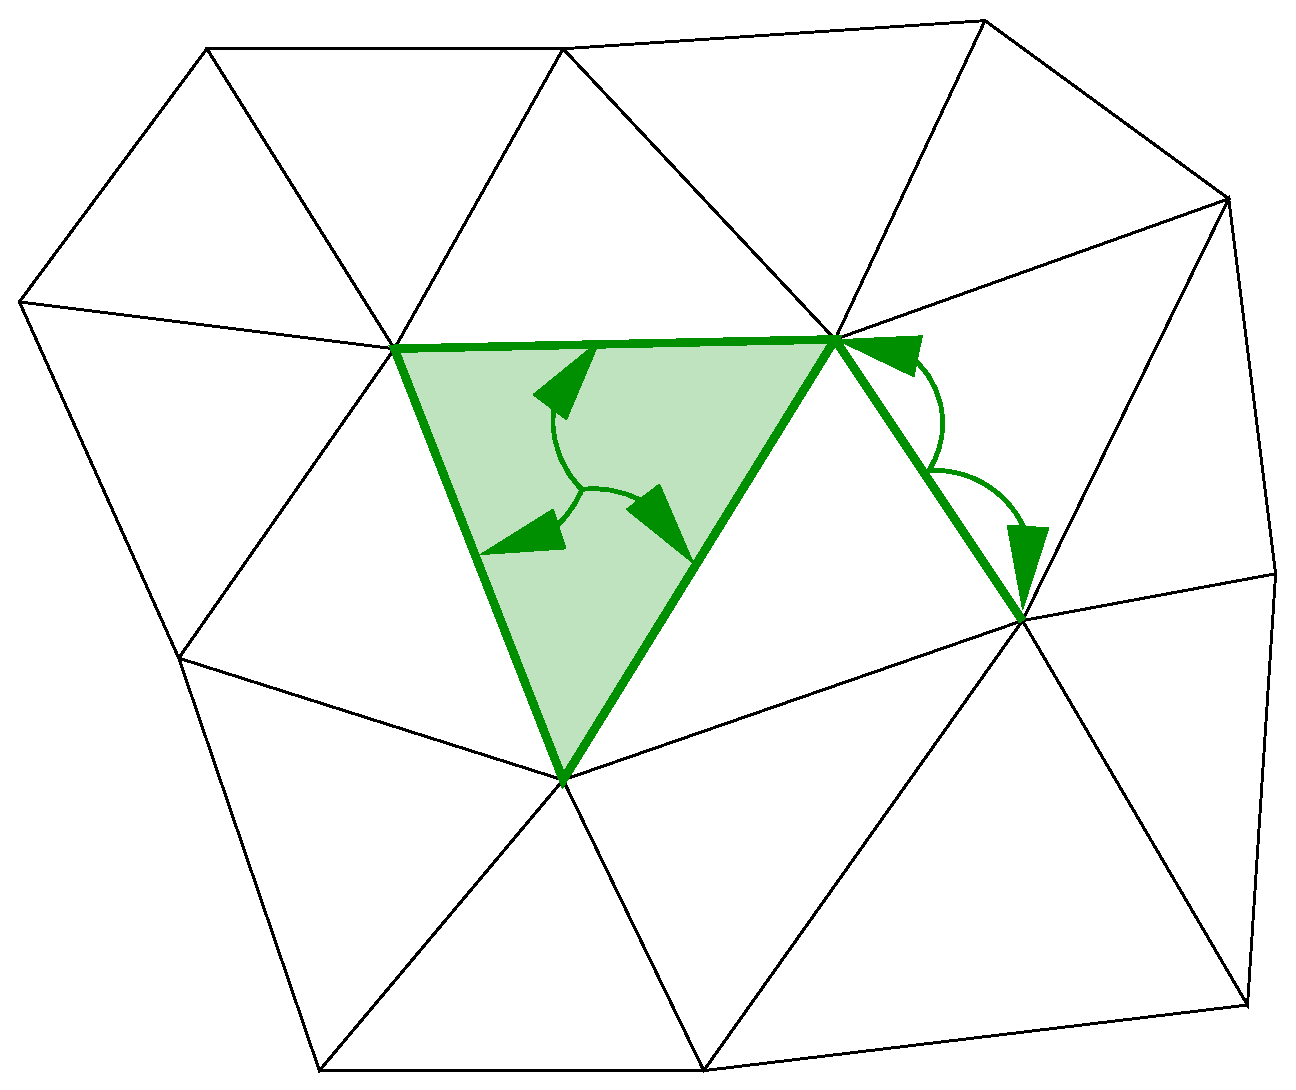
\includegraphics[width=0.3\textwidth]{pics/downward}

}\hfill{}\subfloat[Upward adjacency: edges adjacent to a vertex, faces adjacent to an
edge.]{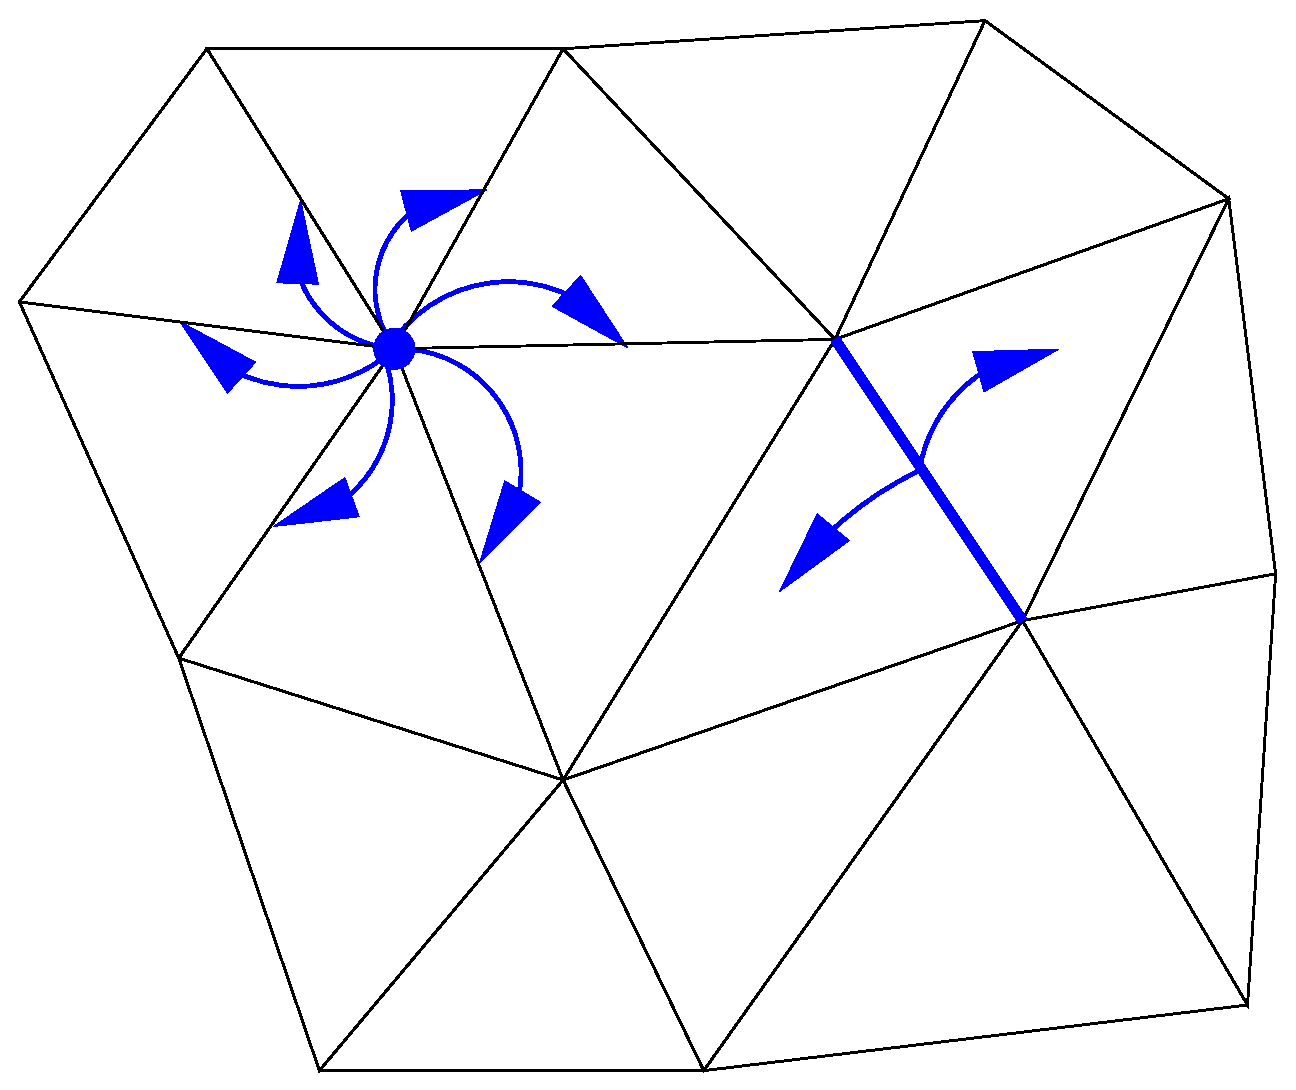
\includegraphics[width=0.3\textwidth]{pics/upward}

}\hfill{}\subfloat[Second adjacency; red edges are adjacent to vertices adjacent to the
red face.]{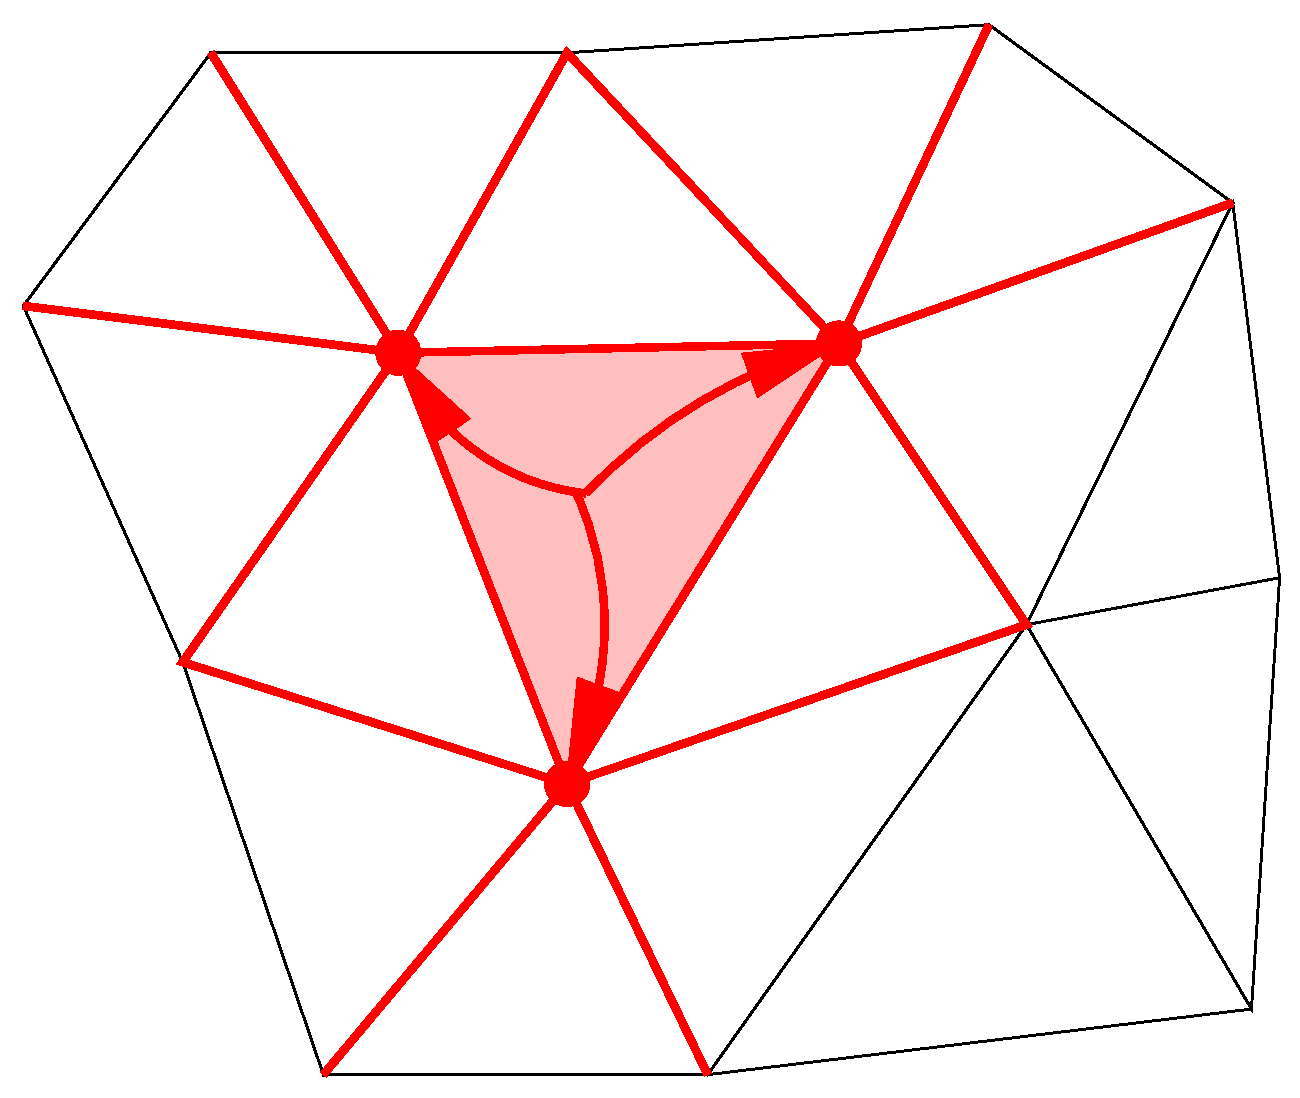
\includegraphics[width=0.3\textwidth]{pics/second}

}

\caption{Examples of adjacency relationships between mesh entities.\label{fig:Adjacency}}

\end{figure}

\par\end{center}


\subsection{Entity Sets}

\label{sub:Entity-Sets}

The iMesh data model allows arbitrary groupings of entities, called
\emph{entity sets}. Each entity set may be a true set (in the set
theoretic sense) or it may be a (possibly non-unique) ordered list
of entities; in the latter case, entities are retrieved in the order
in which they were added to the entity set. An entity set may or may
not be a simply-connected computational mesh; entity sets that \emph{are}
simple meshes have obvious application in multiblock and multigrid
contexts, for instance. Entity sets (other than the root set) are
populated by addition or removal of entities from the set. In addition,
set Boolean operations --- subtraction, intersection, and union ---
on entity sets are also supported.

Two primary relationships among entity sets are supported. First,
entity sets may contain one or more entity sets (by definition, all
entity sets belong to the root set). An entity set contained in another
may be either a subset or an element (each in the set theoretic sense)
of that entity set. The choice between these two interpretations is
left to the application; the iMesh component does not impose either
interpretation. Set contents can be queried recursively or non-recursively;
in the former case, if entity set A is contained in entity set B,
a request for the contents of B will include the entities in A (and
the entities in sets contained in A). Second, parent/child relationships
between entity sets are used to represent logical relationships between
sets, including multigrid and adaptive mesh sequences. These logical
relationships naturally form a directed, acyclic graph.

Examples of entity sets include the ordered list of vertices bounding
a geometric face, the set of all mesh faces that lie on that geometric
face, the set of regions assigned to a single processor by mesh partitioning,
and the set of all entities in a given level of a multigrid mesh sequence.

For use with most solution applications, information in the root set
or one or more of its constituent entity sets is typically a valid
mesh for some scientific computing task, examples of which include:
\begin{itemize}
\item A non-overlapping, connected set of iMesh entities; for example, the
structured and unstructured meshes commonly used in finite element
simulations (\emph{simple mesh}). 
\item Overlapping grids in which a collection of simple meshes are used
to represent some portion of the computational domain, including chimera,
multiblock, and multigrid meshes (\emph{multiple mesh}). The interfaces
presented here handle these mesh types in a general way; higher-level
services may be added later to support specific functionalities needed
by these meshes. In this case, each of the simple meshes is a valid
computational mesh, stored as an entity set. 
\item Adaptive meshes in which all entities in a sequence of refined (simple
or multiple) meshes are retained in the root set. The most highly
refined adaptation level typically comprises a simple or multiple
mesh. Typically, different levels of mesh adaptation will be represented
by different entity sets, with many of the entities shared by multiple
entity sets. 
\item Smooth particle hydrodynamic (SPH) meshes, which consist of a collection
of iMesh vertices with no connectivity or adjacency information. 
\end{itemize}
Meshing applications will typically have a valid computational mesh
as their end product, though during processing the mesh database will
often not be in this state.


\subsection{Tags}

\label{sub:Tags}

Tags are used as containers for user-defined data that can be attached
to iMesh entities and entity sets. Different values of a particular
tag can be associated with different entities or sets; for instance,
a boundary condition tag will have different values for an inflow
boundary than for a no-slip wall, and no value at all for faces in
the interior of the mesh. In the general case, iMesh tags do not have
a predefined type and allow the user to attach arbitrary data to mesh
entities; this data is stored and retrieved by implementations as
a byte pattern. To improve performance and ease of use, we support
three specialized tag types: integers, doubles, and entity handles.
These typed tags enable an iMesh implementation to correctly save
and restore tag data when a mesh is written to a file.


\section{Interface Functionality}

\label{sec:Interface-Functionality}

The iMesh interface supports a variety of commonly needed functionalities
for mesh and entity query, mesh modification, entity set operations,
and tags. All data passed through the interface is in the form of
opaque handles to objects defined in the data model. In this section
we describe the functionality available through the iMesh interface.%
\footnote{Note that these descriptions do not include detailed syntax, which
can be found in the interface user guide~\cite{iBase-UG,iMesh-UG}.
Also, note that all function names in the interface are prepended
by iMesh\_; this prefix is omitted in the tables in this paper for
compactness.%
} For a reference implementation and simple usage examples, see the
ITAPS web site~\cite{itaps:http}.


\subsection{Global Queries}

\label{sub:Mesh-Interface}

Global query functions can be categorized into two groups: 1) \emph{database
functions}, that manipulate the properties of the database as a whole
and 2) \emph{set query functions}, that query the contents of entity
sets as a whole; these functions require an entity set argument, which
may be the root set. These functions are summarized in Table~\ref{table:Mesh-Int}.

%
\begin{table}
\caption{Functions for Global Queries. (All function names are prepended with
iMesh\_.)\label{table:Mesh-Int} }


\centering{}\begin{tabular}{|p{1.25in}|p{223pt}|}
\hline 
{\scriptsize Function}  & {\scriptsize Description}\tabularnewline
\hline
\hline 
{\scriptsize newMesh}  & {\scriptsize Creates a new, empty mesh instance}\tabularnewline
\hline 
{\scriptsize dtor}  & {\scriptsize Destroys a mesh instance}\tabularnewline
\hline 
{\scriptsize load}  & {\scriptsize Loads mesh data from file into entity set}\tabularnewline
\hline 
{\scriptsize save}  & {\scriptsize Saves data from entity set to file}\tabularnewline
\hline 
{\scriptsize getRootSet}  & {\scriptsize Returns handle for the root set}\tabularnewline
\hline 
{\scriptsize getGeometricDim}  & {\scriptsize Returns geometric dimension of mesh}\tabularnewline
\hline 
{\scriptsize setGeometricDim}  & {\scriptsize Sets geometric dimension of mesh (must not contain data
yet)}\tabularnewline
\hline 
{\scriptsize getDfltStorage}  & {\scriptsize Tells whether implementation prefers blocked or interleaved
coordinate data}\tabularnewline
\hline 
{\scriptsize getAdjTable}  & {\scriptsize Returns table indicating availability and cost of entity
adjacency data}\tabularnewline
\hline 
{\scriptsize setAdjTable}  & {\scriptsize Specifies requirements for entity adjacencies and iterators}\tabularnewline
\hline 
{\scriptsize areEHValid}  & {\scriptsize Returns true if EH remain unchanged since last user-requested
status reset}\tabularnewline
\hline
\hline 
{\scriptsize getNumOfType}  & {\scriptsize Returns number of entities of type in ES}\tabularnewline
\hline 
{\scriptsize getNumOfTopo}  & {\scriptsize Returns number of entities of topo in ES}\tabularnewline
\hline 
{\scriptsize getEntities}  & {\scriptsize Returns all entities in ES of the given type and topology}\tabularnewline
\hline 
{\scriptsize getVtxArrCoords}  & {\scriptsize For all input vertex handles, return coords; storage
order can be user-specified.}\tabularnewline
\hline 
{\scriptsize getAdjEntIndices} & {\scriptsize Given ES and optionally a type or topology, return: EH's
in ES of the specified type or topology; EH's adjacent to those entities
with a specified type, as a list of unique handles; and for each entity
in the first list, the adjacent entities specified as indices into
the second list. }\tabularnewline
\hline
\end{tabular}
\end{table}


Database functions include functions to create and destroy mesh instances;
note that the create function only sets up data structures for the
mesh instance, which must be filled by reading data from a file or
by creating a mesh entity by entity. The load and save functions read
and write mesh information from files; file format and read/write
options are implementation dependent. As mesh data is loaded, entities
are stored in the root set, and can optionally be placed into a subsidiary
entity set as well. iMesh implementations must be able to provide
coordinate information in both blocked (xxx...yyy...zzz...) and interleaved
(xyzxyzxyz...) formats; an application can query the implementation
to determine the implementation's preferred storage order. 

For a particular implementation, not all first-order adjacencies are
necessarily available. For instance, in a classic finite element element-node
connectivity storage, requests for faces or edges adjacent to an entity
may return nothing, because the implementation has no stored data
to return. For first-order adjacencies that are available in the implementation,
the implementation may store the adjacency information directly, or
compute adjacencies by either a local traversal of the entity's neighborhood
or by global traversal of the entity set. Each iMesh implementation
must provide information about the availability and relative cost
of first-order adjacency queries. Also, a service or application may
specify which adjacencies it requires and what entity types it will
iterate over; this information, which can be updated by the service
or application as its needs change, can be used by implementations
to optimize internal storage for minimum memory use and efficient
data retrieval.

Set query functions allow an application to retrieve information about
entities in a set. The entity set may be the root set, which will
return selected contents of the entire database, or may be any subsidiary
entity set. For example, functions exist to request the number of
mesh entities of a given type or topology; the types and topologies
are defined as enumerations. Applications can request handles for
all entities of a given type or topology or handles for entities of
a given type adjacent to all entities of a given type or topology.
Also, vertex coordinates are available in either blocked or interleaved
order. Coordinate requests can be made for the arrays of vertex handles
returned by an adjacency call. Finally, for entities of a given type
and topology, their adjacent entities of a given type can be returned,
along with an array of compressed sparse row style indices into the
global vertex coordinate array can be obtained for both entity and
adjacent entity requests.


\subsection{Entity- and Array-Based Query}

\label{sub:Ent-Interface}

%
\begin{table}
\caption{Functions for Single Entity Queries. (All function names are prepended
with iMesh\_.)\label{table:Entity}}


\centering{}\begin{tabular}{|p{1.25in}|p{223pt}|}
\hline 
{\scriptsize Function}  & {\scriptsize Description}\tabularnewline
\hline
\hline 
{\scriptsize initEntIter}  & {\scriptsize Create an iterator to traverse entities of type and topo
in ES; return true if any entities exist}\tabularnewline
\hline 
{\scriptsize getNextEntIter}  & {\scriptsize Return true and a handle to next entity if there is one;
false otherwise}\tabularnewline
\hline 
{\scriptsize resetEntIter}  & {\scriptsize Reset iterator to restart traverse from the first entity}\tabularnewline
\hline 
{\scriptsize endEntIter}  & {\scriptsize Destroy iterator}\tabularnewline
\hline
\hline 
{\scriptsize getEntType}  & {\scriptsize Return type of entity}\tabularnewline
\hline 
{\scriptsize getEntTopo}  & {\scriptsize Return topology of entity}\tabularnewline
\hline 
{\scriptsize getVtxCoord}  & {\scriptsize Return coordinates of a vertex}\tabularnewline
\hline 
{\scriptsize getEntAdj}  & {\scriptsize Return entities of given type adjacent to EH}\tabularnewline
\hline 
{\scriptsize getEnt2ndAdj}  & {\scriptsize Return entities of given type adjacent to entities of
a second type adjacent to EH}\tabularnewline
\hline
\end{tabular}
\end{table}


%
\begin{table}
\caption{Functions for Block Entity Queries. (All function names are prepended
with iMesh\_.)\label{table:EntArr}}


\centering{}\begin{tabular}{|p{1.25in}|p{223pt}|}
\hline 
{\scriptsize Function}  & {\scriptsize Description}\tabularnewline
\hline
\hline 
{\scriptsize initEntArrIter}  & {\scriptsize Create a block iterator to traverse entities of type
and topo in ES}\tabularnewline
\hline 
{\scriptsize getNextEntArrIter}  & {\scriptsize Return true and a block of handles if there are any;
false otherwise}\tabularnewline
\hline 
{\scriptsize resetEntArrIter}  & {\scriptsize Reset block iterator to restart traverse from the first
entity}\tabularnewline
\hline 
{\scriptsize endEntArrIter}  & {\scriptsize Destroy block iterator}\tabularnewline
\hline
\hline 
{\scriptsize getEntArrType}  & {\scriptsize Return type of each entity}\tabularnewline
\hline 
{\scriptsize getEntArrTopo}  & {\scriptsize Return topology of each entity}\tabularnewline
\hline 
{\scriptsize getEntArrAdj}  & {\scriptsize Return entities of type adjacent to each EH}\tabularnewline
\hline 
{\scriptsize getEntArr2ndAdj}  & {\scriptsize Return entities of given type adjacent to entities of
a second type adjacent to each EH}\tabularnewline
\hline
\end{tabular}
\end{table}


The global queries described in the previous section are used to retrieve
information about all entities in an entity set. While this is certainly
a practical alternative for some types of problems and for small problem
size, larger problems or situations involving mesh modification require
access to single entities or to blocks of entities. The iMesh interface
supports traversal and query functions for single entities and for
blocks of entities; the query functions supported are entity type
and topology, vertex coordinates, and entity adjacencies. Blocks of
data are passed through the interface using arrays of entity handles.
Tables~\ref{table:Entity} and~\ref{table:EntArr} summarize these
functions.


\subsection{Mesh Modification}

\label{sub:Mesh-Modification}

The iMesh interface supports mesh modification by providing a minimal
set of operators for low-level modification; both single entity (see
Table~\ref{table:Modify}) and block versions (see Table~\ref{table:ModArr})
of these operators are provided. High-level functionality, including
mesh generation, quality assessment, and validity checking, can in
principle be built from these operators, although in practice such
functionality is more likely to be provided using intermediate-level
services that perform complete unit operations, including vertex insertion
and deletion with topology updates, edge and face swapping, and vertex
smoothing.

%
\begin{table}
\caption{Functions for Single Entity Mesh Modification. (All function names
are prepended with iMesh\_.)\label{table:Modify}}


\centering{}\begin{tabular}{|p{1.25in}|p{223pt}|}
\hline 
{\scriptsize Function}  & {\scriptsize Description}\tabularnewline
\hline
\hline 
{\scriptsize createVtx}  & {\scriptsize Create vertex at given location}\tabularnewline
\hline 
{\scriptsize setVtxCoords}  & {\scriptsize Changes coordinates of existing vertex}\tabularnewline
\hline 
{\scriptsize createEnt}  & {\scriptsize Create entity of given topology from lower-dimensional
entities; return entity handle and creation status}\tabularnewline
\hline 
{\scriptsize deleteEnt}  & {\scriptsize Delete EH from the mesh}\tabularnewline
\hline
\end{tabular}
\end{table}


%
\begin{table}
\caption{Functions for Block Mesh Modification. (All function names are prepended
with iMesh\_.)\label{table:ModArr}}


\centering{}\begin{tabular}{|p{1.25in}|p{223pt}|}
\hline 
{\scriptsize Function}  & {\scriptsize Description}\tabularnewline
\hline
\hline 
{\scriptsize createVtxArr}  & {\scriptsize Create vertices at given location}\tabularnewline
\hline 
{\scriptsize setVtxArrCoords}  & {\scriptsize Changes coordinates of existing vertices}\tabularnewline
\hline 
{\scriptsize createEntArr}  & {\scriptsize Create entities of given topology from lower-dimensional
entities; return entity handle and status}\tabularnewline
\hline 
{\scriptsize deleteEntArr}  & {\scriptsize Delete each EH from the mesh}\tabularnewline
\hline
\end{tabular}
\end{table}


Geometry modification is achieved through functions that change vertex
locations. Vertex locations are set at creation, and can be changed
as required, for instance, by mesh smoothing or other vertex movement
algorithms.

Topology modification is achieved through the creation and deletion
of mesh entities. Creation of higher-dimensional entities requires
specification, in canonical order, of an appropriate collection of
lower-dimensional entities. For instance, a tetrahedron can be created
using four vertices, six edges or four faces, but not from combinations
of these. Upon creation, adjacency information properly connecting
the new entity to its closure is set up by the implementation. Some
implementations may allow the creation of duplicate entities (for
example, two edges connecting the same two vertices), while others
will respond to such a creation request by returning a copy of the
already-existing entity.

Deletion of existing entities is typically done from highest to lowest
dimension. The iMesh interface also allows the deletion of an entity
with existing upward adjacencies (for instance, an edge that is still
in use by one or more faces or regions); in this case, downward adjacency
requests may be nonsensical.




\subsection{Entity Sets}

\label{sub:Entity-Set-Interface}

Entity set functionality in the iMesh interface is divided into three
parts: basic set functionality, hierarchical set relations, and set
Boolean operations.

%
\begin{table}
\caption{Functions for Basic Entity Set Functionality. (All function names
are prepended with iMesh\_.)\label{table:EntSet}}


\centering{}\begin{tabular}{|p{1.25in}|p{223pt}|}
\hline 
{\scriptsize Function}  & {\scriptsize Description}\tabularnewline
\hline
\hline 
{\scriptsize createEntSet}  & {\scriptsize Creates a new entity set (ordered and non-unique if isList
is true)}\tabularnewline
\hline 
{\scriptsize destroyEntSet}  & {\scriptsize Destroys existing entity set}\tabularnewline
\hline 
{\scriptsize isList}  & {\scriptsize Return true if the set is ordered and non-unique}\tabularnewline
\hline
\hline 
{\scriptsize getNumEntSets}  & {\scriptsize Returns number of entity sets contained in SH}\tabularnewline
\hline 
{\scriptsize getEntSets}  & {\scriptsize Returns entity sets contained in SH}\tabularnewline
\hline 
{\scriptsize addEntSet}  & {\scriptsize Adds entity set SH1 as a member of SH2}\tabularnewline
\hline 
{\scriptsize rmvEntSet}  & {\scriptsize Removes entity set SH1 as a member of SH2}\tabularnewline
\hline 
{\scriptsize isEntSetContained}  & {\scriptsize Returns true if SH2 is a member of SH1}\tabularnewline
\hline
\hline 
{\scriptsize addEntToSet}  & {\scriptsize Add entity EH to set SH}\tabularnewline
\hline 
{\scriptsize rmvEntFromSet}  & {\scriptsize Remove entity EH from set SH}\tabularnewline
\hline 
{\scriptsize addEntArrToSet}  & {\scriptsize Add array of entities to set SH}\tabularnewline
\hline 
{\scriptsize rmvEntArrFromSet}  & {\scriptsize Remove array of entities from set SH}\tabularnewline
\hline 
{\scriptsize isEntContained}  & {\scriptsize Returns true if EH is a member of SH}\tabularnewline
\hline 
{\scriptsize isEntArrContained}  & {\scriptsize Check an array of entities for membership in SH}\tabularnewline
\hline
\end{tabular}
\end{table}


Basic set functionality, summarized in Table~\ref{table:EntSet},
includes creating and destroying entity sets; adding and removing
entities and sets; and several entity set specific query functions.%
\footnote{Note that the global mesh query functions (Section~\ref{sub:Mesh-Interface})
and traversal functions (Section~\ref{sub:Ent-Interface}) defined
above can be used with the root set or any other entity set as their
first argument.%
} Entity sets can be either ordered and non-unique, or unordered and
unique; an ordered set guarantees that set query results (including
traversal) will always be given in the order in which entities were
added to the set. The ordered/unordered status of an entity set must
be specified when the set is created and can be queried.

Entity sets are created empty. Entities can be added to or removed
from the set individually or in blocks; for ordered sets, the last
of a number of duplicate entries will be the first to be deleted.
Also, entity sets can be added to or removed from each other; note
that, because all entities and sets are automatically contained in
the root set from creation, calls that would add or remove an entity
or set from the root set are not permitted. An entity set can also
be queried to determine the number and handles of sets that it contains,
and to determine whether a given entity or set belongs to that set.

%
\begin{table}
\caption{Functions for Entity Set Relationships. (All function names are prepended
with iMesh\_.)\label{table:SetRel}}


\centering{}\begin{tabular}{|p{1.25in}|p{223pt}|}
\hline 
{\scriptsize Function}  & {\scriptsize Description}\tabularnewline
\hline
\hline 
{\scriptsize addPrntChld}  & {\scriptsize Create a parent (SH1) to child (SH2) relationship}\tabularnewline
\hline 
{\scriptsize rmvPrntChld}  & {\scriptsize Remove a parent (SH1) to child (SH2) relationship}\tabularnewline
\hline 
{\scriptsize isChildOf}  & {\scriptsize Return true if SH2 is a child of SH1}\tabularnewline
\hline 
{\scriptsize getNumChld}  & {\scriptsize Return number of children of SH}\tabularnewline
\hline 
{\scriptsize getChldn}  & {\scriptsize Return children of SH}\tabularnewline
\hline 
{\scriptsize getNumPrnt}  & {\scriptsize Return number of parents of SH}\tabularnewline
\hline 
{\scriptsize getPrnts}  & {\scriptsize Return parents of SH}\tabularnewline
\hline
\end{tabular}
\end{table}


Hierarchical relationships between entity sets are intended to describe,
for example, multilevel meshes and mesh refinement hierarchies. The
directional relationships implied here are labeled as parent-child
relationships in the iMesh interface. Functions are provided to add,
remove, count, and identify parents and children and to determine
if one set is a child of another; see Table~\ref{table:SetRel}.

%
\begin{table}
\caption{Functions for Entity Set Boolean Operations. (All function names are
prepended with iMesh\_.)\label{table:SetBool}}


\centering{}\begin{tabular}{|p{1.25in}|p{223pt}|}
\hline 
{\scriptsize Function}  & {\scriptsize Description}\tabularnewline
\hline
\hline 
{\scriptsize subtract}  & {\scriptsize Return set difference SH1-SH2 in SH}\tabularnewline
\hline 
{\scriptsize intersect}  & {\scriptsize Return set intersection of SH1 and SH2 in SH}\tabularnewline
\hline 
{\scriptsize unite}  & {\scriptsize Return set union of SH1 and SH2 in SH}\tabularnewline
\hline
\end{tabular}
\end{table}


Set Boolean operations --- intersection, union, and subtraction ---
are also defined by the iMesh interface; these functions are summarized
in Table~\ref{table:SetBool}. The definitions are intended to be
compatible with their C++ standard template library (STL) counterparts,
both for semantic clarity and so that STL algorithms can be used by
implementations where appropriate. All set Boolean operations apply
not only to \emph{entity} members of the set, but also to \emph{set}
members. Note that set hierarchical relationships are not included:
the set resulting from a set Boolean operation on sets with hierarchical
relationships will \emph{not} have any hierarchical relationships
defined for it, regardless of the input data. For instance, if one
were to take the intersection of two directionally-coarsened meshes
(stored as sets) with the same parent mesh (also a set) in a multigrid
hierarchy, there is no reason to expect that the resulting set will
necessarily be placed in the multigrid hierarchy at all. On the other
hand, if both of those directionally-coarsened meshes contain a set
of boundary faces, then their intersection will contain that set as
well.

While set Boolean operations are completely unambiguous for unordered
entity sets, ordered sets make things more complicated. For operations
in which one set is ordered and one unordered, the result set is unordered;
its contents are the same as if an unordered set were created with
the (unique) contents of the ordered set and the operation were then
performed. In the case of two ordered sets, the iMesh specification
tries to follow the spirit of the STL definition, with complications
related to the possibility of multiple copies of a given entity handle
in each set. We recognize that these rules are somewhat arbitrary,
but have been unable to find a more systematic way of defining these
operations for ordered sets. In the following discussion, assume that
a given entity handle appears $m$ times in the first set and $n$
times in the second set.
\begin{itemize}
\item For intersection of two ordered sets, the output set will contain
$\min\left(m,n\right)$ copies of the entity handle. These will appear
in the same order as in the first input set, with the first copies
of the handle surviving. For example, intersection of the two sets
$A=\textrm{\{$abacdbca$\}}$ and $B=\{dadbac\}$ will result in $A\bigcap B=\{abacd\}$. 
\item Union of two ordered sets is easy: the output set is a concatenation
of the input sets: $A\bigcup B=\{abacdbcadadbac\}$. 
\item Subtraction of two ordered sets results in a set containing $\max\left(m-n,0\right)$
copies of an entity handle. These will appear in the same order as
in the first input set, with the first copies of the handle surviving.
For example, $A-B=\{abc\}$. 
\end{itemize}
Regardless of whether the entity members of an entity set are ordered
or unordered, the set members are always unordered and unique, with
correspondingly simple semantics for Boolean operations.


\subsection{Tags}

\label{sub:Tag-Interface}

%
\begin{table}
\caption{Basic Tag Functions. (All function names are prepended with iMesh\_.)\label{table:Tags}}


\centering{}\begin{tabular}{|p{1.25in}|p{223pt}|}
\hline 
{\scriptsize Name}  & {\scriptsize Description}\tabularnewline
\hline
\hline 
{\scriptsize createTag}  & {\scriptsize Creates a new tag of the given type and number of values}\tabularnewline
\hline 
{\scriptsize destroyTag}  & {\scriptsize Destroys the tag if no entity is using it or if force
is true}\tabularnewline
\hline
\hline 
{\scriptsize getTagName}  & {\scriptsize Returns tag ID string}\tabularnewline
\hline 
{\scriptsize getTagSizeValues}  & {\scriptsize Returns tag size in number of values}\tabularnewline
\hline 
{\scriptsize getTagSizeBytes}  & {\scriptsize Returns tag size in number of bytes}\tabularnewline
\hline 
{\scriptsize getTagHandle}  & {\scriptsize Return tag with given ID string, if it exists}\tabularnewline
\hline 
{\scriptsize getTagType}  & {\scriptsize Return data type of this tag}\tabularnewline
\hline
\hline 
{\scriptsize getAllTags}  & {\scriptsize Return handles of all tags associated with entity EH}\tabularnewline
\hline 
{\scriptsize getAllEntSetTags}  & {\scriptsize Return handles of all tags associated with entity set
SH}\tabularnewline
\hline
\end{tabular}
\end{table}


Tags are used to associate application-dependent data with a mesh,
entity, or entity set. Basic tag functionality defined in the iMesh
interface is summarized in Table~\ref{table:Tags}, while functionality
for setting, getting, and removing tag data is summarized in Table~\ref{table:Tags2}.

When creating a tag, the application must provide its data type and
size, as well as a unique name. For generic tag data, the tag size
specifies how many bytes of data to store; for other cases, the size
tells how many values of that data type will be stored. The implementation
is expected to manage the memory needed to store tag data. The name
string and data size can be retrieved based on the tag's handle, and
the tag handle can be found from its name. Also, all tags associated
with a particular entity can be retrieved; this can be particularly
useful in saving or copying a mesh.

%
\begin{table}
\caption{Setting, Getting, and Removing Tag Data. (All function names are prepended
with iMesh\_.)\label{table:Tags2}}


\centering{}\begin{tabular}{|p{1.25in}|p{223pt}|}
\hline 
{\scriptsize Function}  & {\scriptsize Description}\tabularnewline
\hline
\hline 
{\scriptsize setData}  & {\scriptsize The value in tag TH for entity EH is set to the first
tagValSize bytes of the array\textless{}char\textgreater{} tagVal}\tabularnewline
\hline 
{\scriptsize setArrData}  & {\scriptsize The value in tag TH for entities in EHarray{[}i{]} is
set using data in the array<char> tagValArray and the tag size}\tabularnewline
\hline 
{\scriptsize setEntSetData}  & {\scriptsize The value in tag TH for entity set SH is set to the first
tagValSize bytes of the array<char> tagVal}\tabularnewline
\hline 
{\scriptsize set{[}Int,Dbl,EH{]}Data}  & {\scriptsize The value in tag TH for entity EH is set to the int,
double, or entity handle in tagVal; array and entity set versions
also exist.}\tabularnewline
\hline 
{\scriptsize getData}  & {\scriptsize Return the value of tag TH for entity EH}\tabularnewline
\hline 
{\scriptsize getArrData}  & {\scriptsize Retrieve the value of tag TH for all entities in EH array,
with data returned as an array of tagVal's}\tabularnewline
\hline 
{\scriptsize getEntSetData}  & {\scriptsize Return the value of tag TH for entity EH}\tabularnewline
\hline 
{\scriptsize get{[}Int,Dbl,EH{]}Data}  & {\scriptsize Return the value of tag TH for entity EH; array and entity
set versions also exist.}\tabularnewline
\hline
\hline 
{\scriptsize rmvTag}  & {\scriptsize Remove tag TH from entity EH}\tabularnewline
\hline 
{\scriptsize rmvArrTag}  & {\scriptsize Remove tag TH from all entities in EH array}\tabularnewline
\hline 
{\scriptsize rmvEntSetTag}  & {\scriptsize Remove tag TH from entity set SH}\tabularnewline
\hline
\end{tabular}
\end{table}


Initially, a tag is not associated with any entity or entity set,
and no tag values exist; association is made explicitly by setting
data for a tag-entity pair. Tag data can be set for single entities,
arrays of entities (each with its own value), or for entity sets.
In each of these cases, separate functions exist for setting generic
tag data and type-specific data. Analogous data retrieval functions
exist for each of these cases.

When an entity or set no longer needs to be associated with a tag
--- for instance, a vertex was tagged for smoothing and the smoothing
operation for that vertex is complete --- the tag can be removed from
that entity without affecting other entities associated with the tag.
When a tag is no longer needed at all --- for instance, when all vertices
have been smoothed --- the tag can be destroyed through one of two
variant mechanisms. First, an application can remove this tag from
all tagged entities, and then request destruction of the tag. Simpler
for the application is forced destruction, in which the tag is destroyed
even though the tag is still associated with mesh entities, and all
tag values and associations are deleted. Some implementations may
not support forced destruction.


\subsection{Error Handling}

\label{sub:Error-Handling}

Like any API, the iMesh interface is vulnerable to errors, either
through incorrect input or through internal failure within an implementation.
For instance, it is an error for an application to request entities
with conflicting types and topologies. Also, an error in the implementation
occurs when memory for a new object cannot be allocated. The iMesh
interface defines a number of standard error conditions which could
occur in iMesh functions, either because of illegal input or internal
implementation errors; each of these error conditions has an accompanying
description, which can be retrieved by calling iMesh\_getDescription,
summarized in Table~\ref{table:Error}.

%
\begin{table}
\caption{Error Handling Functionality. (All function names are prepended with
iMesh\_.)\label{table:Error}}


\centering{}\begin{tabular}{|p{1.25in}|p{223pt}|}
\hline 
{\scriptsize Name}  & {\scriptsize Description}\tabularnewline
\hline
\hline 
{\scriptsize getDescription}  & {\scriptsize Retrieves error description}\tabularnewline
\hline
\end{tabular}
\end{table}



\subsection{Compliance Testing}

\label{sub:Compliance-Testing}

To ensure consistency between implementations and to assist users
developing partial implementations based on their own mesh data structures,
we have developed a comprehensive compliance test suite for the iMesh
interface. When testing a full implementation of the interface, the
test suite uses the iMesh implementation to read a mesh file, then
tests each interface function. These tests are typically done by comparing
information retrieved in multiple ways --- for instance, retrieving
coordinate information in both blocked and interleaved order, or retrieving
adjacency information entity-by-entity or for all entities of a given
type. The set and tag functions can be easily tested by creating sets
or tags in the test code and querying the new sets and tags to verify
their correctness. We are currently working on a function-level compliance
testing, so that users wishing to use a single iMesh-based service
can implement and test only the functions required for that service.
This fine-grained testing is much more difficult, because consistency
between different calls can no longer be relied on. The combination
of these two test suites will ensure that different iMesh implementations
have the same behavior, and that applications can rely on correct
interaction with iMesh services.


\subsection{Fortran Compatibility}

\label{sub:Fortran-Compatibility}

For compatibility with the Fortran convention that functions returning
values do not modify their arguments, no iMesh function returns a
value. That is, all iMesh functions are C void functions or Fortran
subroutines. Also, string arguments in the C API have an accompanying
argument giving their length; these string length arguments are added
at the end of the argument list in the order the strings appear. Fortran77
and Fortran90/95 compilers must support the pass-by-value extension
to be compatible with the iMesh API. Fortran 2003 has C interoperability
features that greatly simply matters; we provide a Fortran 2003 module
definition and examples online~\cite{itaps:http}.


\section{Usage Examples}

\label{sec:Usage-Examples}

In this section, we provide several examples of using the iMesh component,
including finite element simulation, mesh modification, mesh partitioning,
and visualization. Each of these services has been demonstrated to
work with multiple implementations of the iMesh component, and ---
where efficiency data are available --- the overhead of using the
iMesh API rather than a native implementation is quite small. In addition
to these examples of direct iMesh usage, members of our consortium
are collaborating with applications researchers to introduce ITAPS
software tools into applications in accelerator design, nuclear fusion,
groundwater simulation, combustion, and computational biology; these
efforts are not described in this paper.


\subsection{Existing iMesh Implementations}

\label{sub:Existing-iMesh-Implementations}

Before discussing applications of the iMesh interface, we will summarize
the status of the existing iMesh implementations. Our consortium has
produced a complete reference implementation of the iMesh interface
as well as four complete implementations based on our pre-existing
mesh databases, all of which are available directly through our website~\cite{itaps:http};
most also have their own websites. Each of the five supports all standard
finite element topologies --- hexahedra, tetrahedra, prisms, pyramids,
triangles, and quadrilaterals. Each has its own particular strengths
and areas of most frequent application. 
\begin{itemize}
\item The reference implementation (RefImpl) is intended as a basic mesh
database with full support for all iMesh functionality. Users looking
for a testbed for experimenting with iMesh or for implementing meshing
algorithms without the difficulties of first writing a mesh database
will find this implementation of particular interest.
\item The Flexible Mesh DataBase (FMDB)~\cite{ReSh03} is designed especially
to handle adaptively changing mesh data, including flexible storage
of adjacency information. Application usage of FMDB includes computational
fluid dynamics (CFD), fusion, and accelerator simulations.
\item The Mesh Oriented datABase (MOAB)~\cite{moab} is particularly efficient
in its memory management. Application usage for MOAB includes nuclear
reactor modeling, neutron transport, and accelerator design optimization.
\item The Generation and Refinement of Unstructured Mixed-element Meshes
in Parallel (GRUMMP)~\cite{GRUMMP:http} toolkit is designed for
triangular/tetrahedral mesh generation, improvement, and adaptation,
and is particularly efficient in retrieving adjacency information.
Application usage is primarily in CFD, especially aerodynamics and
non-Newtonian fluid dynamics.
\item The Pacific Northwest National Laboratory's NWGRID~\cite{nwgrid:http}
is intended for adaptive mesh refinement, especially for simplicial
meshes. Application usage includes computational biology, CFD, solid
mechanics, and subsurface transport modeling.
\end{itemize}

\subsection{A Simple Finite Element Solver}

\label{sub:FESolve}

To demonstrate the cost of using the iMesh interface in a typical
computational science application, we developed a simple finite element
application that solves a diffusion problem in two dimensions on the
unit square:

\begin{equation}
\nabla(k\nabla u(x,y))=f\end{equation}
 \begin{equation}
u(x=0)=0\quad u(x=1)=1\quad u_{x}(y=0)=0\quad u_{x}(y=1)=0.\end{equation}
The finite element solver uses linear triangular elements and exact
integration rules. The finite element solver is written in C and uses
PETSc to solve the linear systems.

We focus our attention on setting up the linear system and consider
four different options for accessing the mesh data: 1) through array-based
mechanisms defined in the iMesh interface, which should approximate
the performance of a native implementation; 2) through entity iterators;
and 3) through entity array iterators. Regardless of access method,
we require for each vertex its coordinates; a global id and a boundary
flag as stored attached to the vertices as tags. For elements, we
require downward adjacency information (face to vertex) and store
a global id and computed element area as tags. We make use of the
iMesh functions given in Table \ref{table:FEfunctions}. In all cases,
we must obtain the root set from the iMesh instance and get the tag
handles for the global ids, boundary flags and element areas. In the
case of array access, we obtain a lists of all the vertex and face
entities in the mesh and can obtain the tag data as arrays of size
\emph{num\_vtx} or \emph{num\_elem}. We can obtain the vertex coordinate
information and element connectivity information using these entity
arrays or, as we did in this example, directly from the mesh data
base. It is guaranteed by the iMesh interface that the information
returned using these array-based calls will have a consistent ordering
across all calls. The iMesh calls used for the entity and entity array
iterators provide the same functionality either entity by entity or
for arrays of entities. In each case, we initialize the iterator to
return mesh faces and get entity information through the getNextEnt(Arr)Iter
function. For each entity (array) returned, we obtain the downward
vertex adjacency information, the vertex coordinates, and needed global
id, boundary, and element area tag data.

%
\begin{table}
\caption{iMesh functions used in the simple finite element solver for different
mesh data access\label{table:FEfunctions}}


\centering{}\begin{tabular}{|p{1.25in}|p{1.25in}|p{1.25in}|}
\hline 
{\scriptsize Array Access}  & {\scriptsize Entity Iterator}  & {\scriptsize Entity Array Iterator}\tabularnewline
\hline
\hline 
{\scriptsize getRootSet}  & {\scriptsize getRootSet}  & {\scriptsize getRootSet} \tabularnewline
{\scriptsize getTagHandle}  & {\scriptsize getTagHandle}  & {\scriptsize getTagHandle} \tabularnewline
{\scriptsize getVtxCoordIndex}  & {\scriptsize initEntIter}  & {\scriptsize initEntArrIter} \tabularnewline
{\scriptsize getAllVtxCoords}  & {\scriptsize getNextEntIter}  & {\scriptsize getNextEntArrIter} \tabularnewline
{\scriptsize getEntities}  & {\scriptsize getEntAdj}  & {\scriptsize getEntArrAdj} \tabularnewline
{\scriptsize getIntArrData}  & {\scriptsize getVtxCoord}  & {\scriptsize getVtxArrCoords} \tabularnewline
{\scriptsize getDblArrData}  & {\scriptsize getIntData}  & {\scriptsize getIntArrData} \tabularnewline
  & {\scriptsize getDblArrData}  & {\scriptsize getDblArrData} \tabularnewline
\hline
\end{tabular}
\end{table}


This application has been timed with two iMesh implementations, GRUMMP
and SimpleMesh, a small-scale test implementation developed at Lawrence
Livermore; the application has also been tested successfully with
other iMesh implementations, although timings are not reported here.
We ran each case 40 times and report the average time required to
set up the linear system in milliseconds, along with the percentage
increase in cost compared to the use of problem-sized arrays, in Table
\ref{table:FEtimes}. In the case of the entity array iterator, we
used array sizes of 1, 3, 5, 10 and 20. This is a small problem size;
the total number of elements in the mesh is 6077, so the largest array
iterator represents only about 0.3\% of the total problem size. Not
surprisingly, the array based access to the vertex and element information
is the fastest. Entity iterators are perhaps the most natural to program,
but result in the highest overhead costs due to the very large number
of function calls ($10+3\cdot(n_{e}+n_{e}\cdot n_{v})+4\cdot n_{v}$),
where $n_{e}$ is the number of elements and $n_{v}$ is the number
of vertices; for the SimpleMesh implementation, the overhead is only
6.6\%, but for the GRUMMP implementation it is a much higher 27.6\%.
The entity array iterator cases decrease in cost as the array size
grows and number of function calls decreases; in this case, the total
number of iMesh function calls is $10+6*n_{e}/\left|WS\right|+4*n_{v}/\left|WS\right|$,
where $\left|WS\right|$ is the size of the work set; for both implementations,
the overhead is reduced by at least a factor of two compared with
entity iterators.

%
\begin{table}[htb]
 

\caption{Timing results for the 2D linear finite element solver using the SimpleMesh
implementation of the iMesh interface.\label{table:FEtimes}}


\centering{}\begin{tabular}{|l||r|r||r|r|}
\hline 
Case  & \multicolumn{2}{c||}{SimpleMesh } & \multicolumn{2}{c|}{GRUMMP}\tabularnewline
\cline{2-5} 
 & Time (ms) & $\frac{(T-T_{\mbox{array}})}{T_{\mbox{array}}}\times100$  & Time (ms) & $\frac{(T-T_{\mbox{array}})}{T_{\mbox{array}}}\times100$ \tabularnewline
\hline
\hline 
Array-based  & 81.8 & ---  & 86.7 & --- \tabularnewline
Entity Iterator  & 87.2 & 6.6\%  & 110.6 & 27.6\%\tabularnewline
Entity Array Iterator (1)  & 87.6 & 7.1\%  & 109.0 &  25.8\%\tabularnewline
Entity Array Iterator (3)  & 86.2 & 6.7\%  & 102.5 &  18.2\%\tabularnewline
Entity Array Iterator (5)  & 85.3 & 4.3\%  & 99.0 &  14.1\%\tabularnewline
Entity Array Iterator (10)  & 85.4 & 4.5\%  & 97.4 &  12.3\%\tabularnewline
Entity Array Iterator (20)  & 84.4 & 3.3\%  & 95.9 &  10.6\%\tabularnewline
\hline
\end{tabular}
\end{table}



\subsection{Mesh Quality Improvement via Vertex Movement}

\label{sec:Mesh-Vert-Opt}

The MESh QUality Improvement Toolkit (Mesquite)\cite{Mesquite03}
improves the accuracy of mesh-based simulations through optimization
of the mesh vertex locations. Mesquite can be used for element shape
optimization, r-adaptivity, mesh alignment, etc., and has been tested
with the MOAB, FMDB, GRUMMP and NWGRID iMesh implementations.

As input Mesquite requires an iMesh instance and entity set handle
designating the subset of the mesh over which to perform the optimization.
If the entity set handle is the root set, optimization is done for
the entire mesh. Further, Mesquite expects an integer tag indicating
whether the corresponding vertex may be moved during optimization.
Generally, boundary vertices are marked as fixed or otherwise constrained
to the computational domain boundary to ensure correct problem formulation.
While there is some variation in iMesh functionality requirements
in the different Mesquite solvers, all Mesquite optimization algorithms
require iteration over elements and vertices contained in an entity
set, element-vertex adjacency queries, entity set creation and modification,%
\footnote{This is an artifact of early versions of both Mesquite and the iMesh
interface. The Mesquite-iMesh interaction code could be updated to
remove the need for this capability.%
} vertex coordinate query and modification, and tag data query. These
capabilities are sufficient to support Mesquite's global element shape
optimizer; a sample input mesh is shown in Figure~\ref{fig:msq-shape}(a)
with the corresponding output mesh in Figure~\ref{fig:msq-shape}(b).
When optimizing a single vertex or subsets of mesh vertices, iMesh
implementation must also efficiently determine the elements adjacent
to a vertex. Output results were identical for both the global and
Laplacian smoothers, and for data access using Mesquite's native mesh
representation and via the iMesh interface.

%
\begin{figure}
\begin{centering}
\subfloat[Initial mesh]{

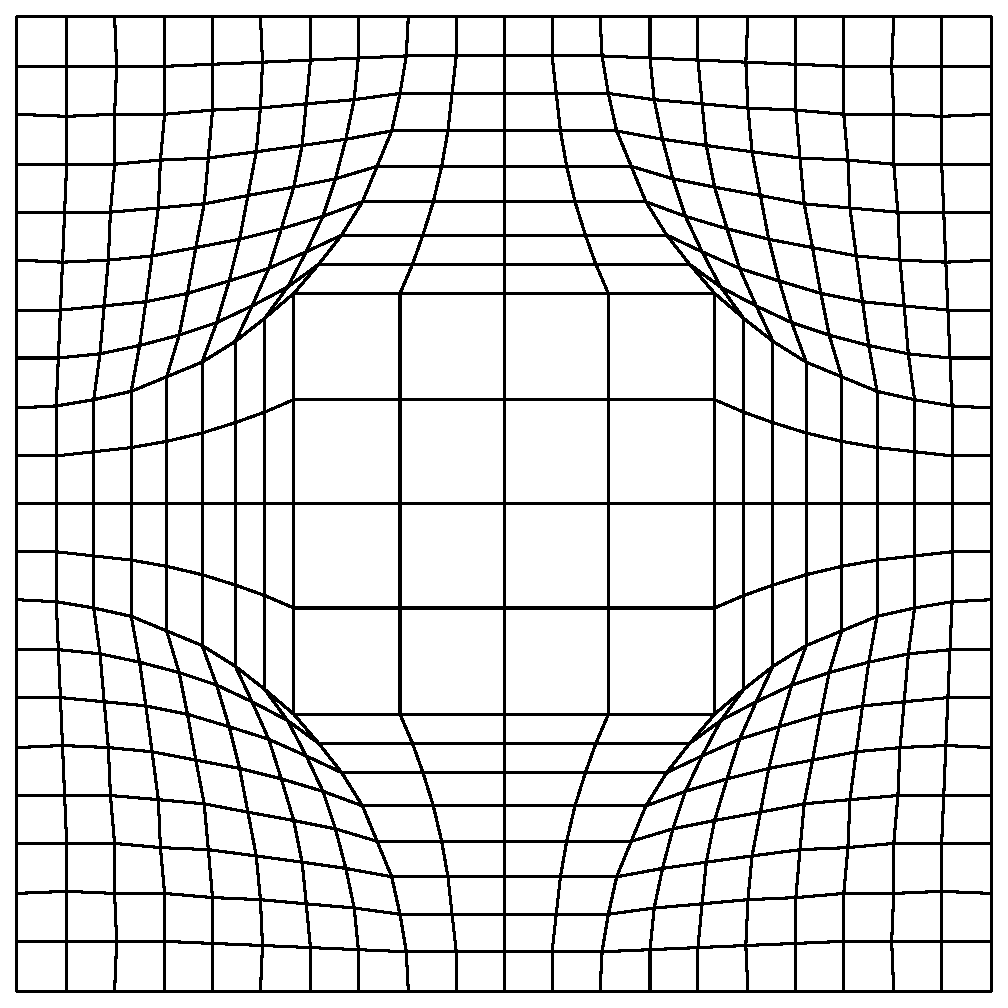
\includegraphics[width=0.3\textwidth]{msq/corners}}\hfill{}\subfloat[Optimized mesh]{

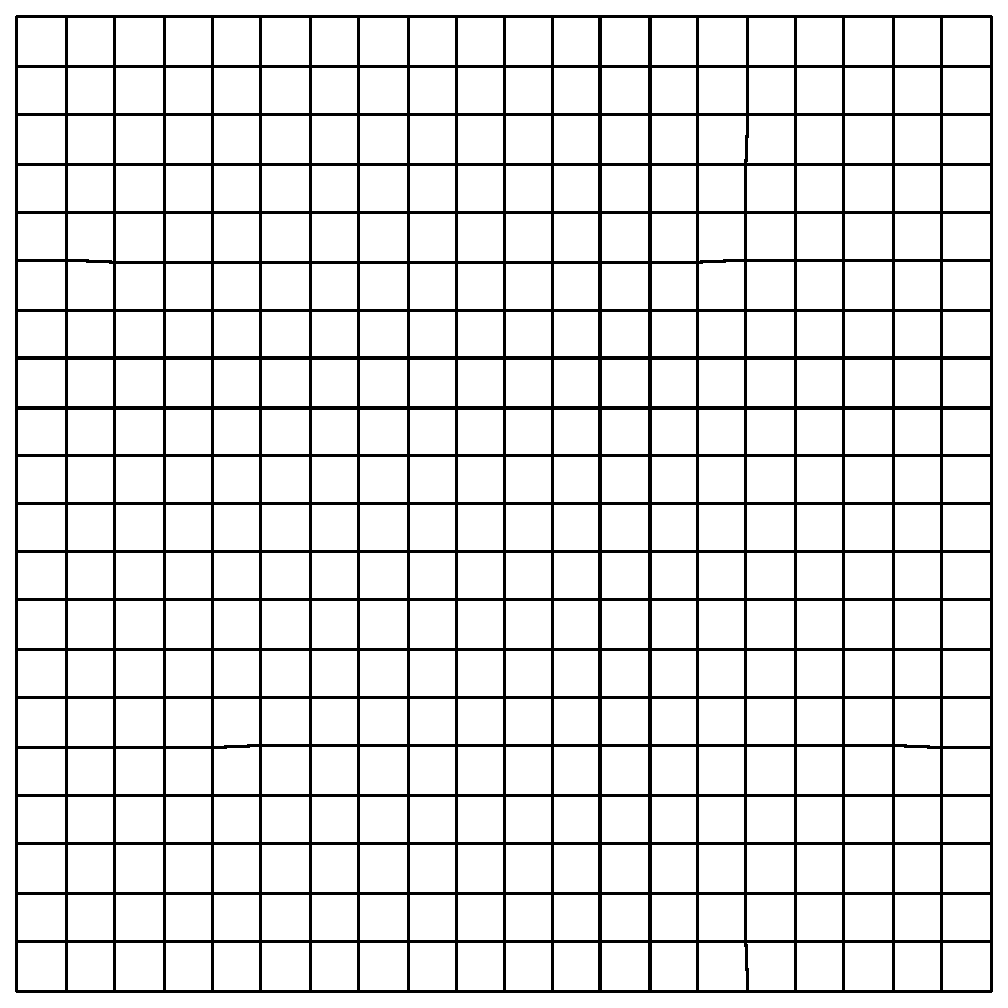
\includegraphics[width=0.3\textwidth]{msq/direct}}\hfill{}\subfloat[Optimized mesh using target matrix optimization]{

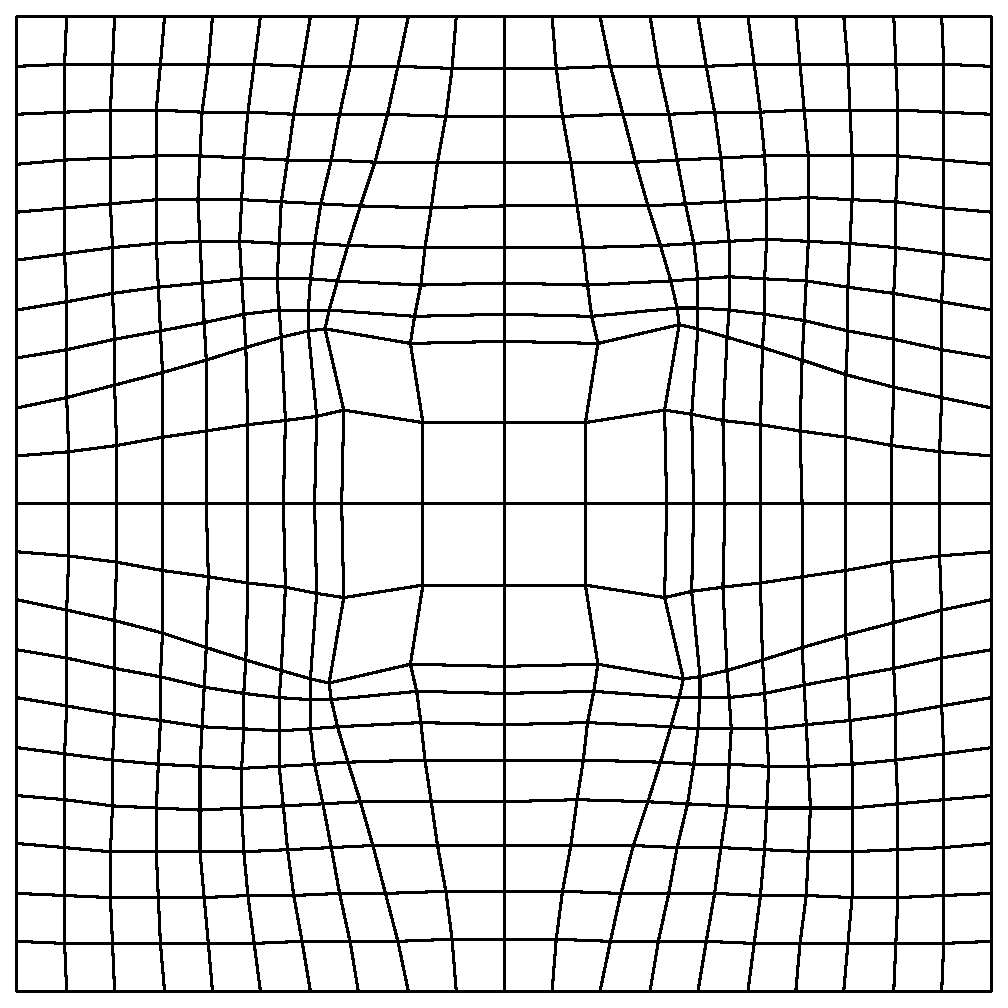
\includegraphics[width=0.3\textwidth]{msq/target}} 
\par\end{centering}

\caption{Element shape optimization using Mesquite.\label{fig:msq-shape}}

\end{figure}


%
\begin{figure}
\begin{centering}
%
\begin{minipage}[c]{0.45\columnwidth}%
\begin{center}
\subfloat[Initial mesh]{\begin{centering}
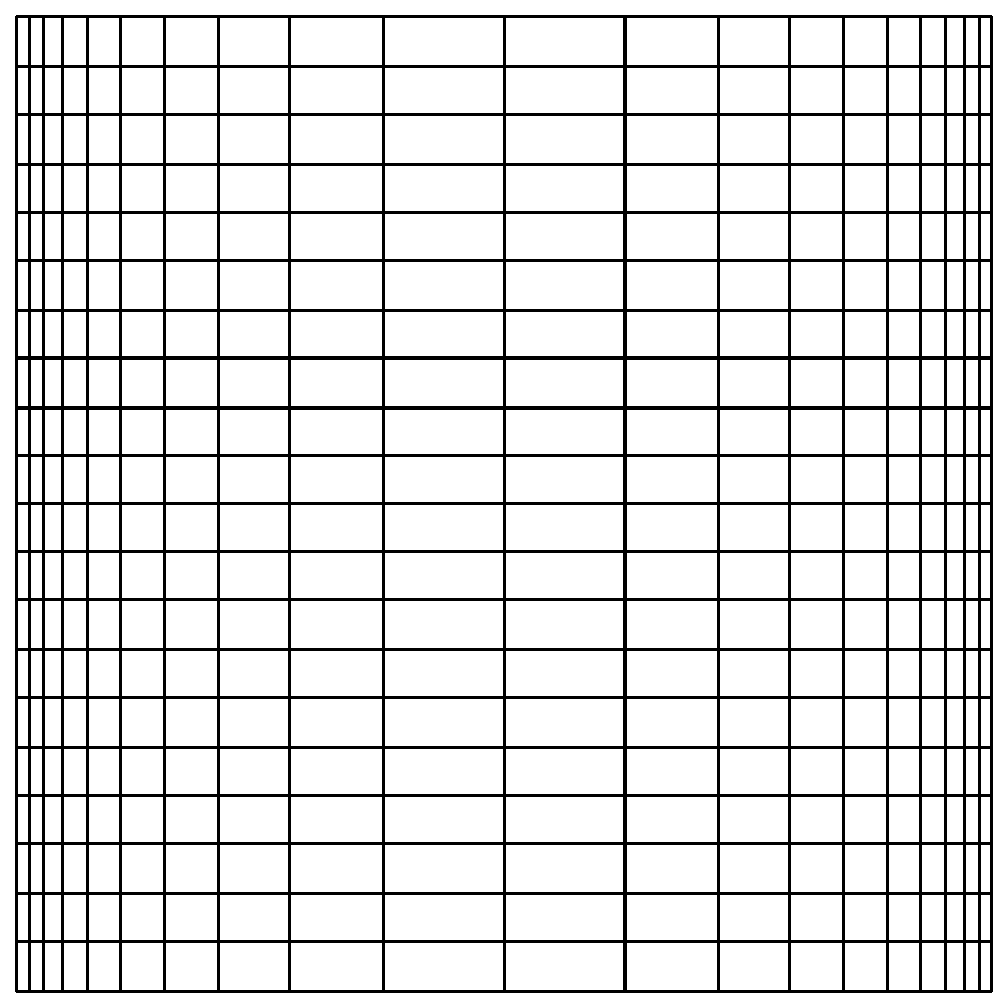
\includegraphics[width=1\textwidth]{msq/bias}
\par\end{centering}

} 
\par\end{center}%
\end{minipage}\hfill{}%
\begin{minipage}[c]{0.45\columnwidth}%
\begin{center}
\subfloat[Deformed mesh]{\begin{centering}
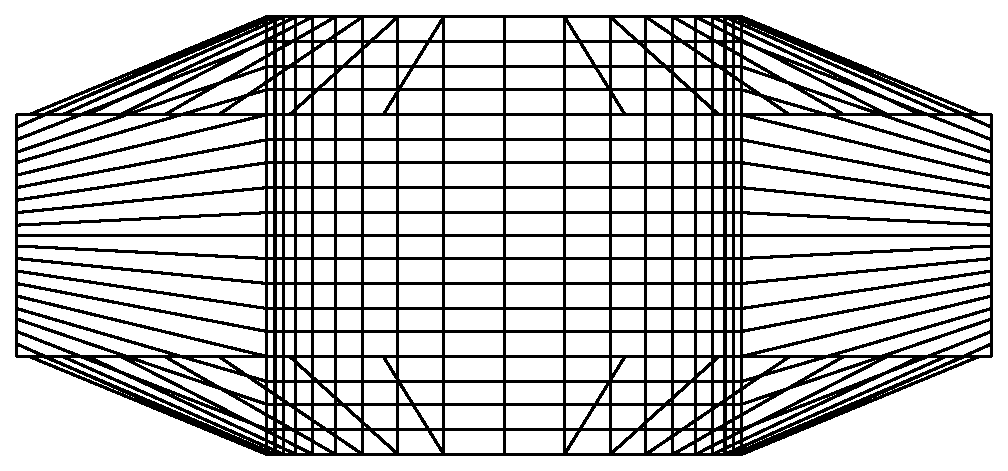
\includegraphics[width=1\textwidth]{msq/deformed}
\par\end{centering}

}
\par\end{center}

\begin{center}
\subfloat[Optimized mesh]{\begin{centering}
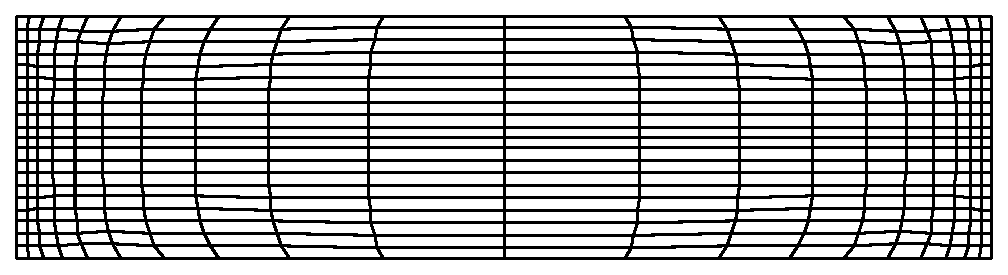
\includegraphics[width=1\textwidth]{msq/def-opt}
\par\end{centering}

}
\par\end{center}%
\end{minipage}
\par\end{centering}

\caption{Deforming boundary optimization using Mesquite.\label{fig:msq-deform}}

\end{figure}


Mesquite is also capable of optimizing to obtain specific characteristics
of the mesh on an element-by-element basis using target matrices.
These pre-calculated target matrices are stored as iMesh tag data
on the mesh elements and retrieved during optimization. For example,
Figure \ref{fig:msq-shape}(c) is the result of optimizing the same
input mesh given previously, except that target matrices are used
to preserve the size and aspect ratio of the elements. Another example
is shown in Figure \ref{fig:msq-deform} in which element aspect ratio
is preserved while updating the mesh for a deforming mesh boundary.
An initial anisotropic mesh, shown in Figure \ref{fig:msq-deform}(a),
is used to calculate the target matrices. Figure \ref{fig:msq-deform}(b)
shows the same mesh after boundary deformation, with some elements
inverted due to the change in location of the boundary vertices. This
mesh (with the stored target matrices) is the input to the Mesquite
optimizer. The resulting mesh, with the element anisotropy preserved,
is shown in Figure \ref{fig:msq-deform}(c).

%
\begin{table}
\caption{CPU Time (seconds) for optimization of 40,000 element meshes.}


\begin{centering}
\label{table:msq-times} 
\par\end{centering}

\centering{}\begin{tabular}{|l|r@{.}l|r@{.}l|r@{.}l|}
\hline 
Optimizer  & \multicolumn{2}{c|}{Internal} & \multicolumn{4}{c|}{iMesh}\tabularnewline
\cline{1-1} \cline{4-7} 
 & \multicolumn{2}{c|}{} & \multicolumn{2}{c|}{MOAB} & \multicolumn{2}{c|}{GRUMMP}\tabularnewline
\hline 
Global shape optimization  & 45  & 38  & 45  & 16  & 45  & 16 \tabularnewline
\hline 
Laplacian smoother  & 111  & 60  & 472  & 65  & \multicolumn{2}{c|}{---}\tabularnewline
\hline 
Target matrix optimization  & 79  & 30  & 82  & 65  & 89  & 38 \tabularnewline
\hline 
Deforming boundary  & 12  & 73  & 15  & 48  & 21  & 59 \tabularnewline
\hline
\end{tabular}
\end{table}


Table \ref{table:msq-times} shows the impact of the iMesh interface
and implementation on optimizer performance.%
\footnote{The iMesh implementation in GRUMMP does not yet support vertex-to-element
adjacency queries for surface meshes, so it was not possible to run
this Laplacian smoothing example with the GRUMMP iMesh implementation.%
} Each row of the table corresponds to one of the examples above with
the mesh interval size reduced by a factor of ten, resulting in meshes
with 40,000 elements. The global shape optimization results demonstrate
one of the advantages of using a mesh database library over a custom
storage scheme. The more compact representation of data in the iMesh
implementations results in a slight performance improvement over Mesquite's
internal mesh representation. The Laplacian smoothing times emphasize
the overhead of a standard interface and generalized mesh database.
The smoothing calculation is trivial. The time spent in tens of millions
of queries for small amounts of data (adjacencies, tag data, vertex
coordinates, etc.) dominates the run time of the optimization. The
latter two rows in Table \ref{table:msq-times} demonstrate the run
time cost of accessing tag data. The time spent accessing other mesh
data is the same as for the global shape optimization case. The difference
in run time for each mesh database is entirely a function of the time
spent querying target matrices stored in tag data.


\subsection{Mesh Quality Improvement via Topology Optimization}

\label{sub:Mesh-Topo-Opt}

Local mesh topology optimization can be a powerful tool for improving
the quality of unstructured meshes; however, mesh topology modification
--- often referred to as swapping --- is difficult enough to implement
that an iMesh-based service that performs these operations would be
useful for many applications. The classic face and edge swapping operations~(see,
for instance,~\cite{Freitag1997} for a description) have been implemented
using the iMesh API~\cite{TSTT-swap-tool}.

The swapping service represents a worst-case scenario for efficiency
tests for the iMesh interface, in that the service requires fine-grained
access to and modification of the mesh database using the interface.
As such, the swapping service makes a large number of calls through
the interface, each returning a small amount of data. Specifically,
the swapping service uses the iMesh entity iterators, adjacency queries,
array-based vertex coordinate queries, checks for entity type and
topology, and entity creation and deletion functions. Optionally,
the swapping service can also be restricted to reconfigure only tetrahedra
that are members of a given set, requiring the ability to query set
membership and to assign new entities to sets. A second optional functionality
is the ability to accept a tag and tag value to indicate which faces
within a set should be considered for swapping.

%
\begin{table}
\caption{Performance for the iMesh swapping service for a supersonic aircraft
mesh (251,140 tetrahedra).\label{tab:swapping-service}}


\begin{centering}
%
\begin{comment}
\begin{center}
\begin{tabular}{|c||c|c|c|c|}
\hline 
 & Native & \multicolumn{3}{c|}{iMesh implementations}\tabularnewline
\cline{3-5} 
 & (non-iMesh)  & GRUMMP  & FMDB  & MOAB\tabularnewline
\hline
\hline 
Swaps  & 25,448  & 28,629  & 27,811  & 27,592\tabularnewline
\hline 
Rate $\left(\frac{1}{\mbox{sec}}\right)$  & 3,380  & 2,800  & 223  & 122\tabularnewline
\hline 
Memory (MB) & 216 MB  & 292 MB & 622 MB & 110 MB\tabularnewline
\hline
\end{tabular}
\par\end{center}
\end{comment}
{}
\par\end{centering}

\centering{}\begin{tabular}{|c||c|c|}
\hline 
 & Native & \multicolumn{1}{c||}{GRUMMP}\tabularnewline
 & (non-iMesh)  & iMesh\tabularnewline
\hline
\hline 
Swaps  & 25,448  & 28,629 \tabularnewline
\hline 
Rate $\left(\frac{1}{\mbox{sec}}\right)$  & 3,380  & 2,800 \tabularnewline
\hline 
Memory (MB) & 216 MB  & 292 MB\tabularnewline
\hline
\end{tabular}
\end{table}


The swapping service has been tested with three different iMesh implementations:
GRUMMP, MOAB, and FMDB, and the results compared with an implementation
of the same algorithms using the GRUMMP back-end (referred to as \emph{native}).
For testing purposes, we use a mesh for a supersonic aircraft initially
containing 251,140 tetrahedra. Because of differences in the order
in which faces are accessed, output meshes from the iMesh swapping
service are not identical but we have confirmed elsewhere~\cite{TSTT-swap-tool}
that the meshes have statistically indistinguishable quality. Table~\ref{tab:swapping-service}
compares the number of swaps performed, the swapping rate, and the
memory used for the native swapping implementation and the swapping
service using the GRUMMP iMesh implementation. The CPU time overhead
for using the GRUMMP iMesh implementation rather than the native implementation
is about 20\% for this case; the 40\% overhead in memory usage is
required to support certain forms of entity creation that are not
supported natively by the mesh database. Preliminary timing results
for the MOAB and FMDB databases suggest that, for this service, good
performance depends on careful attention to optimization of frequently-called
iMesh functions, especially iterators and adjacency retrieval; in
some cases, design decisions in the mesh database may also have a
significant impact on performance. %
\begin{comment}
Table~\ref{tab:swapping-service} contains the number of swaps performed,
the swapping rate, and the memory used for each implementation. The
CPU time overhead for using the GRUMMP iMesh implementation rather
than the native implementation is about 20\% for this case; the 40\%
overhead in memory usage is required to support certain forms of entity
creation that are not supported natively by the mesh database. The
results for this case clearly show that the designers of the FMDB
and MOAB mesh databases made different trade-offs in deciding what
data to store and how. MOAB was designed for low memory usage ---
less than 40\% of the memory usage of the next smallest database here.
FMDB was designed for parallel performance and flexibility, neither
of which are required by this service. Figure~\ref{fig:cpu-breakdown}
shows relative CPU time for each implementation, broken down into
the time spent in the swapping service itself; retrieving adjacency
information; retrieving coordinate information; performing mesh modifications;
reading and pre-processing mesh data; and manipulating iterators.
The difference in relative cost for the swapping service reflects
the difference in total CPU time, as the absolute time for the driver
varies by only about 10\% between implementations. The most significant
differences in overall performance are clearly in adjacency retrieval
and iterators. Optimization of these routines would no doubt improve
their performance significantly for this service and others that use
the iMesh interface similarly. This case also illustrates clearly
that efficient implementation of iMesh functions that are used heavily
by a service is essential for good run-time performance.

%
\begin{figure}
\caption{Breakdown of relative CPU time for the swapping service with three
different iMesh implementations\label{fig:cpu-breakdown}}


\centering{}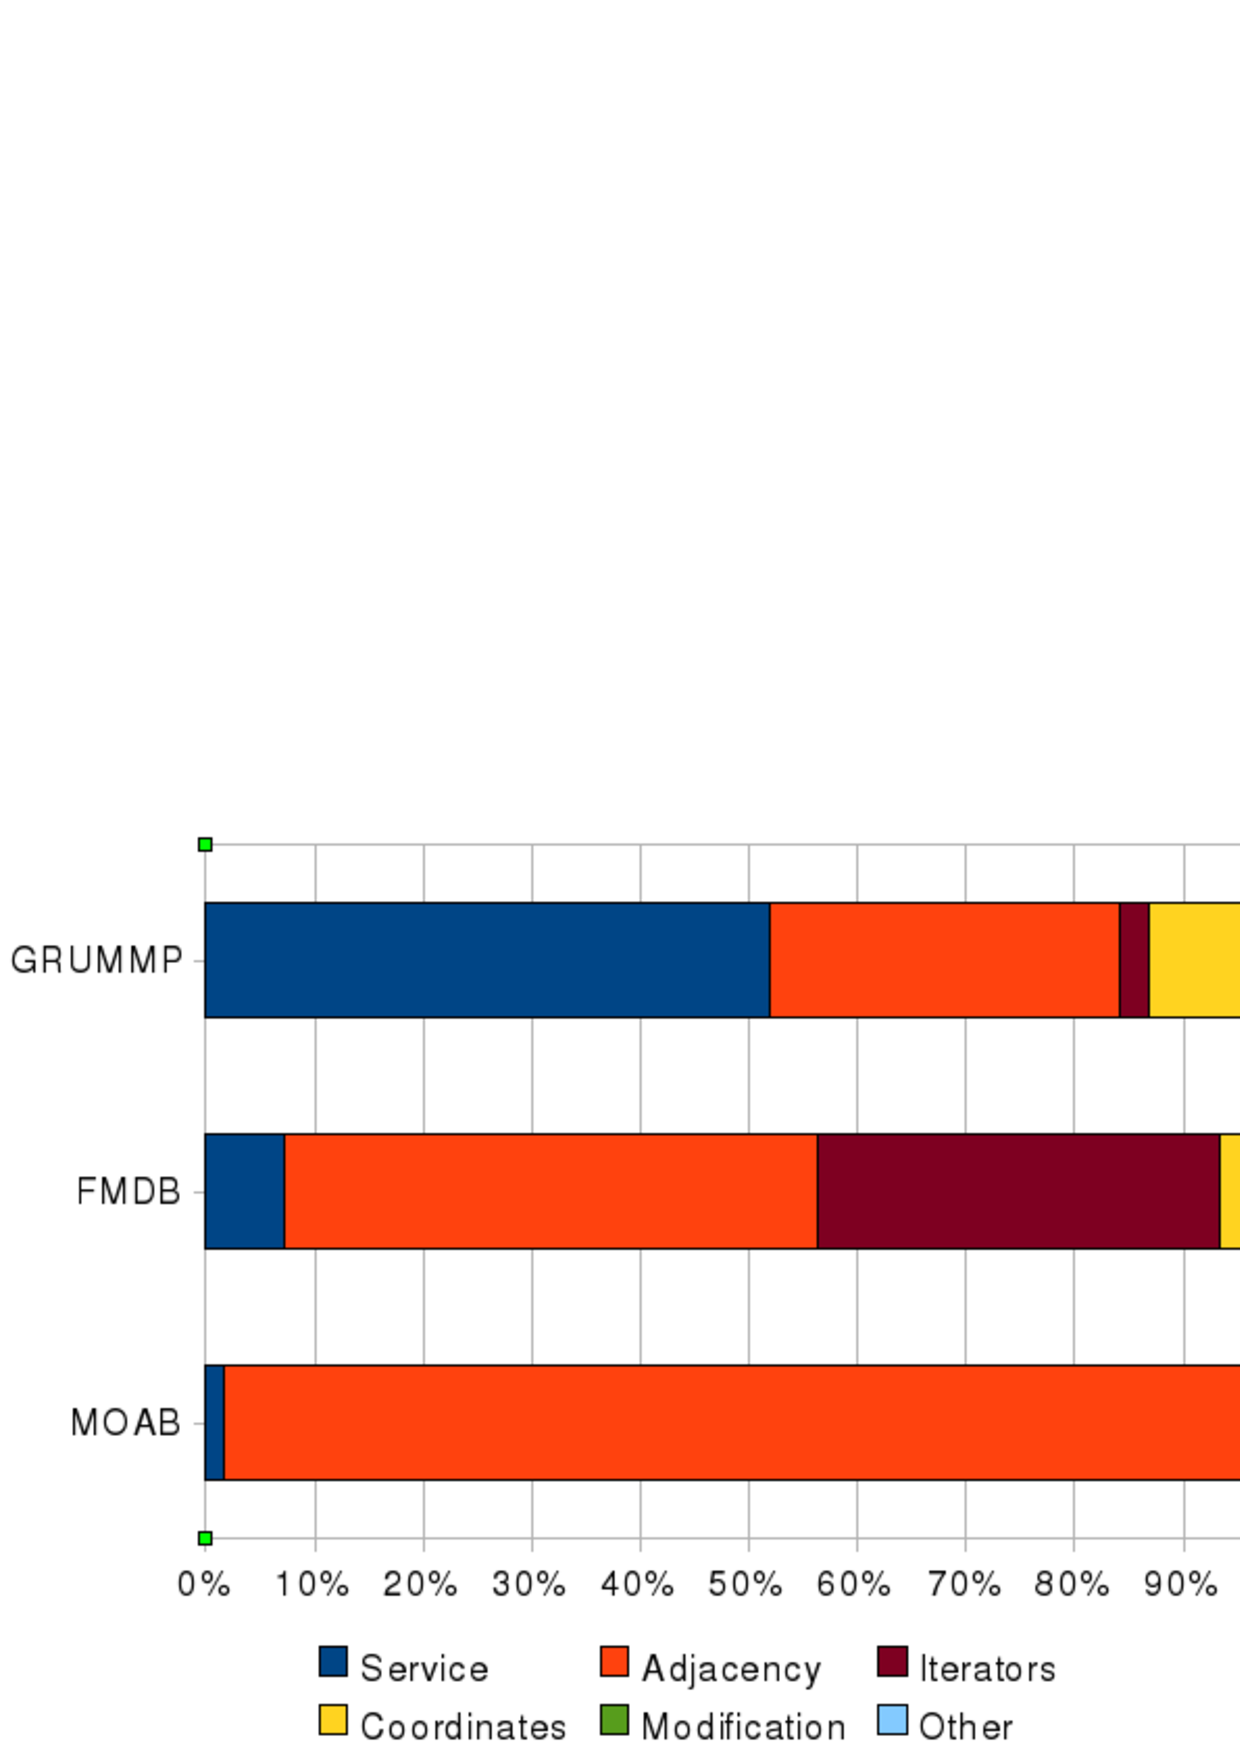
\includegraphics[width=0.7\textwidth]{pics/time-bar.png} 
\end{figure}

\end{comment}
{}


\subsection{A Partitioning Service}

As a precursor to our ongoing work for a parallel extension to the
iMesh interface, an iMesh-based service that performs partitioning
would be useful. Partitioning distributes data over sets of processors
and is needed by unstructured and/or adaptive parallel applications.
Many of the partitioning methods in Zoltan~\cite{Zoltan} have been
made available in a service that uses the iMesh API to access mesh
data. The partitioners available can be grouped into three categories;
simple partitioners for testing and demonstration, geometric or coordinate-based
partitioners, and graph partitioning.

For the simple partitioners, the partitioning service uses the iMesh
queries for entities and number of entities. The partition service
can operate at the level of any mesh entity (i.e. vertex, edge, face,
or region). The partitioning service uses both single-entity and array-of-entities
access to mesh data. For the geometric partitioners, the partitioning
service uses the iMesh single-entity adjacency queries and array-based
vertex coordinate queries. For graph partitioning, the partitioning
service uses the array-based adjacency queries.

The partition data is stored by both attaching an integer tag to each
mesh entity and collecting entities into sets with integer tags. Any
previous partition data is destroyed before new partition data is
created. The partition service uses entity set query, deletion, and
creation functions as well as the ability to assign new entities to
sets and get, destroy, create, and set tag data.

The partitioning service has been tested and is interoperable with
three mesh database implementations available through the iMesh C
interface: MOAB, FMDB, and GRUMMP. Users need only link in the desired
implementation; no other changes are necessary. A partitioning service
interfacing directly to MOAB performs only slightly faster than the
partitioning service interfacing to MOAB through iMesh. To partition
a mesh with 1.4 million faces by faces using recursive coordinate
bisection, the MOAB native implementation required 37.2 seconds, while
using the ITAPS C interface to access the MOAB data structures required
38.2 seconds (2.5\% overhead).


\subsection{Visualization Using the iMesh Interface}

Visualization and interactive manipulation of meshes as well as fields
defined on meshes is important in many aspects of simulation software
development. Towards this end, we have developed a VisIt~\cite{VisIt2005}
plugin that accesses mesh and solution data through an iMesh implementation.
We have demonstrated that the current plugin is interoperable across
three different iMesh implementations: GRUMMP, MOAB and FMDB. The
plugin uses array-based vertex coordinate queries. Solution data is
retrieved using iMesh tag capabilities. In addition, the plugin uses
recursive entity set queries to map an iMesh entity set hierarchy
to a roughly equivalent VisIt construct called a \emph{subset inclusion
lattice}. This enables VisIt to provide intuitive GUI controls to
users in terms of subsets that are characteristic to various stages
of their design and analysis workflows. For example, users often need
to focus their attention on a specific part in the original CAD model,
a specific regime in the material model, or a specific discretization
region in the numerical model. The ability for users to interactively
visualize, query, calculate and otherwise analyze data in terms of
characteristic subsets such as these both within and across each stage
of a design and analysis workflow fundamentally enhances the flexibility
of the analysis activities possible within the VisIt visualization
tool.


\subsection{Size Field-Based Mesh Adaptation}

Adaptive methods are central to ensuring the accuracy and reliability
of simulation results. One approach to supporting mesh adaptation
is to provide a service that can take an existing mesh with a new
mesh size field associated with it and create the desired adapted
mesh by applying appropriate mesh modification operations. Such a
service for anisotropic mesh adaptation has been under development
of a number of years~\cite{LiSh05}. To ensure the ability to deal
with general curved geometries that can come from CAD systems, the
service builds on a generalized interaction with the geometric model~\cite{BeWa04}
and ensures the mesh can properly represent the domain of interest~\cite{LiSh03}.
This service has been used to construct adaptive simulation procedures
by combining it with finite element and finite volume solvers, and
associated error indicators. Since the mesh adaptation service works
off a general anisotropic mesh size field, error indicators that have
been used include various combinations of analytic fields, anisotropic
\emph{a posteriori} correction indicators and geometric approximation
considerations~\cite{ShFl05,WaKo05}. An example of a part before
and after refinement using this approach is shown in Figure~\ref{fig:adaptation}.

%
\begin{figure}
\subfloat[Before refinement (408 regions)]{

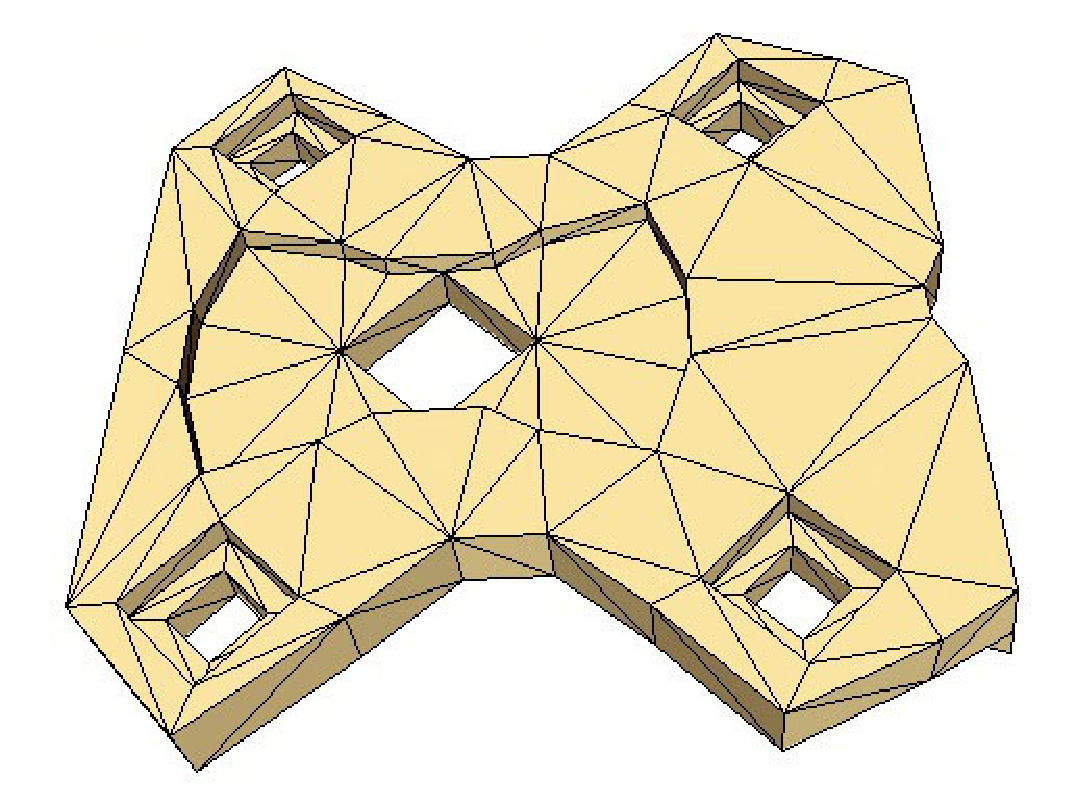
\includegraphics[width=0.4\textwidth]{pics/coarse}}\hfill{}\subfloat[After refinement (36,261 regions)]{

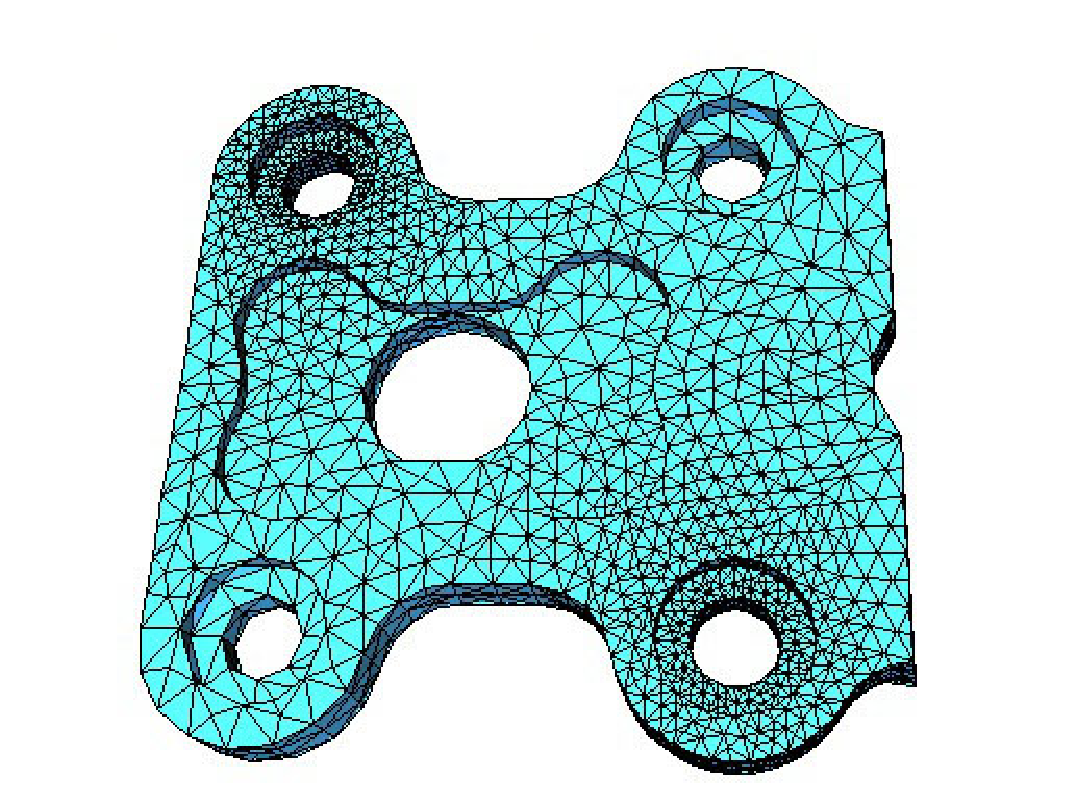
\includegraphics[width=0.4\textwidth]{pics/refined}}

\caption{An example of size field-based mesh adaptation.\label{fig:adaptation}}



\end{figure}


The current version of the mesh adaptation service builds on the FMDB
mesh library that employs mesh topology like iMesh. Although it is
possible to replace all FMDB calls with iMesh calls in the mesh adaptation
service code (an activity planned for the future), the size of the
code and the desire to apply the mesh adaptation to applications quickly
prompted us to take an alternative initial approach. In this approach,
meshes are accessed through the iMesh functions and loaded into the
FMDB structures. The mesh adaptation process is carried out and the
resulting mesh is then put back into iMesh form. This approach has
the disadvantage that at the beginning and end of the mesh adaptation
process there are two copies of the mesh. However, since the size
of the mesh is typically small compared to the structures used during
the implicit finite element and finite volume solvers being used to
date, there have not been memory limitations introduced by this process.


\section{Discussion and Conclusions}

\label{sec:Discussion-and-Conclusions}

In this paper, we have described a new software component for mesh-based
applications --- both meshing and solver applications. We have described
in detail the key features of this software component, called iMesh:
its data model --- which defines the types of data that the component
works with --- and its interface --- which defines how applications
can interact with mesh data.

Also, we have shown by example that iMesh component  is flexible enough
for a wide range of applications --- including finite element solvers,
mesh improvement and adaptation, partitioning, and visualization.
Our experience with these examples shows that relatively complex mesh
modification and solution requirements can be met by the interface,
with low impact on efficiency. Specifically, for a simple finite element
solver, overhead induced by using the iMesh interface is less than
10\%, especially when data for multiple entities is retrieved through
the mesh interface at once. For mesh smoothing, the overhead rate
varied significantly from case to case, depending on the amount of
work done by the smoothing code relative to the number of calls through
the mesh interface. For mesh swapping, another fine-grained use case
for the mesh component, overhead rates were about 20\% compared with
a native implementation of the same algorithms. Three higher-level
services --- mesh partitioning, visualization, and mesh adaptation
--- have also been tested across multiple iMesh implementations. In
each case, the services have proved to be interoperable, and the overhead
in using the iMesh interface is acceptable. Overall, our experience
with these services confirms that relatively complex mesh operations
can be performed correctly using the iMesh interface. Also, we have
found clear examples of significant differences between mesh database
designs in overall run time for a particular service.%
\footnote{Note that this is not contradictory with our finding of low overhead
when comparing native and iMesh-based implementations, as the overhead
measurements compare an iMesh implementation of a service to a non-iMesh
implementation of that same functionality \emph{for a given mesh database}.%
}

Several implementations of the iMesh component are currently available,
as are the services described in this paper.\cite{itaps:http} An
analogous software component for geometric query and manipulation
for mesh-based applications has also been developed, and work is nearing
completion on a parallel extension of the mesh component.


\subsection*{Acknowledgments}

The authors would like to acknowledge the contributions of Kyle Chand
and Tamara Dahlgren (Lawrence Livermore National Laboratories); Seegyoung
Seol (Renssalaer Polytechnic Institute); Xiaolin Li and Brian Fix
(Stony Brook University); and Harold Trease (Pacific Northwest National
Laboratory) to the development of the ITAPS mesh component.

This work was funded by the U.S. Department of Energy under the Scientific
Discovery through Advanced Computing (SciDAC) program and by the Canadian
Natural Sciences and Engineering Research Council under a Special
Research Opportunities grant.

\bibliographystyle{acmtrans}
\bibliography{/home/cfog/ITAPS/repository/Papers/biblio/tstt}

\end{document}
